\documentclass[11pt,a4paper]{article}

% -------- Encoding & language ----------
\usepackage[T1]{fontenc}
\usepackage[utf8]{inputenc}
\usepackage[english]{babel}
\usepackage{lmodern}

% -------- Core maths & symbols ---------
\usepackage{amsmath,amssymb,gensymb}
\usepackage{textcomp}
\usepackage{siunitx}

% -------- Floats, graphics, tables -----
\usepackage{graphicx}           % figures
\usepackage{float}              % [H] specifier
\usepackage{caption}
\usepackage{subcaption}
\captionsetup{justification=centering,singlelinecheck=false,labelfont=bf}
\usepackage{booktabs,tabularx,array,makecell,multirow}
\renewcommand\tabularxcolumn[1]{>{\Centering}m{#1}}
\newcolumntype{L}[1]{>{\raggedright\arraybackslash}p{#1}}
%\renewcommand\tabularxcolumn[1]{>{\centering\arraybackslash}m{#1}}

% -------- Algorithms (choose ONE set) --
\usepackage[linesnumbered,ruled,vlined]{algorithm2e}
% \usepackage{algorithm}        % comment this out if you keep algorithm2e
% \usepackage{algpseudocode}

% -------- Code listings ---------------
\usepackage{minted}             % needs -shell-escape

% -------- Miscellaneous ---------------
\usepackage{hyperref}
\hypersetup{
  colorlinks=true,
  linkcolor=black,
  citecolor=black,
  urlcolor=blue,
  pdftitle={X-jaw},
  pdfpagemode=FullScreen,
}
\usepackage{cleveref}
\usepackage{setspace,enumitem,fancyhdr,ragged2e,indentfirst}
\usepackage{geometry}
\geometry{margin=2.5cm}
\usepackage{csquotes}

% -------- Bibliography -----------------
\usepackage[sorting=none,backend=biber]{biblatex}
\addbibresource{biblio.bib}

% -------- Header / footer --------------
\fancyhf{}
\fancyhead[R]{De Groot}
\fancyfoot[L]{EPFL}
\fancyfoot[C]{\thepage}
\fancyfoot[R]{CREATE Lab}
\renewcommand{\footrulewidth}{0.4pt}
\pagestyle{fancy}
\setlength{\headheight}{14pt}

% -------- Custom commands --------------
\newcommand{\diff}{\mathrm{d}}
\DeclareCaptionLabelFormat{andtable}{#1~#2  \&  \tablename~\thetable}

\setlength{\parskip}{8pt}
\setlength{\parindent}{0pt}

\begin{document}
    \begin{titlepage}
    \newcommand{\HRule}{\rule{\linewidth}{0.2mm}}
    \center
    
\includegraphics[scale=0.25]{figures/logo.png}\\[0.4cm]

    \textsc{\Large École Polytechnique Fédérale de Lausanne}\\[1.5cm]
    \vfill
    
    \HRule \\[0.4cm]
    {\LARGE \bfseries Towards replicating the full chewing process : Initial development of a Stewart platform-based chewing robot.}\\
    \HRule \\ [0.5cm]
    
    \textsc{\Large Master thesis}
    \vfill 
   
    \centering
    \bigskip
    \textit{Author} : \\[0.2cm]

    Barbara \textsc{De Groot, 296815}\\

    \bigskip
    \bigskip

    CREATE Lab, Prof. Josie Hughes\\
    \textit{Supervisor} : Benhui Dai\\[0.2cm]

    \bigskip
    \bigskip
    
    {\large \today}\\[2cm]
    \end{titlepage}

\newpage
\tableofcontents

\newpage
%\input{Abstract}
\section{Introduction}

Human chewing is a complex process, involving different systems such as the jaw, teeth, tongue and saliva, all coordinated to break down food into 
a bolus that can be swallowed and digested. Chewing robots are a great tool to study this process that is not yet fully understood as they give us the opportunity 
for a closely controlled environment where each parameter can be adjusted and measured. This makes them valuable not only for advancing our understanding of 
chewing mechanics and related disorders, but also for a wide range of applications. In dentistry, they are used to test how implants and other dental devices
 wear over time. In food science, they help assess texture and flavor release during mastication. They also offer a reliable platform for studying the release of 
 active compounds in chewable medications such as medical chewing gum.\\
Nowadays, many mastication robots exist, and while most are limited in their ability to fully mimic human chewing due to restricted degrees of freedom, 
some have already made significant progress. For example, the Bristol Dento-Munch Robo-Simulator \cite{BristolChewingRobot} features 6 degrees of freedom 
(DoF), closed-loop control, force feedback, and a full set of teeth capable of replicating human chewing forces. Similarly, the robot developed by Seung-Ju 
Lee \cite{ChewingRobotLinearActuator} offers the same capabilities, with a design that more closely follows human biomechanics. Another system, by Alemzadeh 
et al. \cite{ChewingRobotGums}, includes a closed mouth and artificial saliva—two important components of realistic mastication—even though it has limited 
sensory feedback. However, none of these systems combine all critical elements: 6 DoF, position and multidirectional force feedback, a closed mouth, and 
saliva. In addition, none of them include a tongue, which plays a crucial role in directing the food towards the molars and mixing it with saliva during 
chewing.\\
This project aims at developing a chewing robot that incorporates all these features, with the goal of replicating the full chewing process as closely as 
possible. As this is the first iteration, the focus is primarily on the mechanical design and the development of a simple, closed-loop, modular, and scalable 
control system that can be extended in future versions. The robot includes a 6-DoF Stewart platform capable of replicating chewing forces, along with 
tri-axial force sensing and position feedback to monitor jaw dynamics in detail. In parallel, we created a first dataset of human chewing motion using 
motion capture, as no publicly available datasets were found. This dataset will serve as a reference for identifying chewing patterns and 
improving control strategies. By laying down a flexible and expandable foundation, this work provides a platform for future integration of key components 
such as artificial saliva flow, an artificial tongue, and adaptive neuromuscular control strategies.



\newpage
\section{Methods}

\subsection{Required workspace and forces --> criteria for design}
\begin{itemize}
    \item max chewing force across literature
    \item max range of motion across literature
\end{itemize}

\subsection{Mechanical design}
\begin{itemize}
    \item goal is to create a robotic jaw that can mimic the motion and force of human chewing 
    \item 6dof stewart platform to be able to mimic the motion of the jaw
    \item linear actuators instead of rotary servo motors to have more efficient force transmission + simpler kinematics + more rigid structure
    \item choice of actuators based on the required force to mimic human chewing (speed less important as jaw can chew even if slow) + required length to 
    reach the desired range of motion + feedback to control in position
    \item choosing the dimensions of the stewart platform based on the size of the actuators + working space of the robot
    \item choice of structure/material to hold upper jaw to be rigid enough to not deform under the forces applied by the actuators 
    \item 3 axis load cells to measure the force applied by the jaw
    \item so far 3d printed teeth/jaw but to be changed in the future
\end{itemize}

\subsection{Control}

%The control layer combines a high-speed microcontroller, a modular C++ codebase, and classical PI loops to deliver real-time motion of 
%the Stewart platform.  Figure~\ref{fig:code_structure} gives the software context, while the full electronics schematic is shown in 
%Fig.~\ref{fig:elec_schematic}.

\subsubsection{Hardware (electronics)}
A Teensy~4.1 (600 MHz ARM Cortex-M7, single-precision FPU) executes the control loop.% at \SI{100}{\hertz}. %? %todo: add ref for the freq/reason
Its key peripherals are:  
\begin{itemize}[nosep]
    \item three \SI{12}{\ampere} dual DC motor drivers (DF Robot) controlling the six linear actuators;
    \item six analogue inputs reading potentiometer position feedback from the linear actuators;
    \item three transmitters for the load cells mounted on top of the maxilla;
    \item an on-board micro-SD slot used for trajectory files and calibration data.
\end{itemize}
A \SI{12}{\volt} AC/DC brick powers the actuators directly; the user's computer supplies \SI{5}{\volt} to the Teensy, which in 
turn sources the \SI{3.3}{\volt} logic rails for the motor drivers and load-cell transmitters.
The full electronics schematic is shown in Fig.~\ref{fig:elec_schematic}.

\begin{figure}[H]
\centering
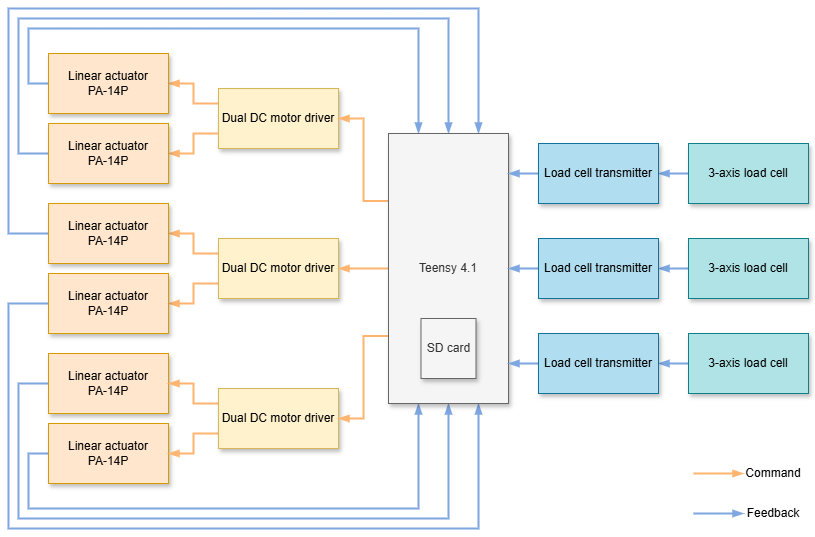
\includegraphics[width=\textwidth]{figures/elec_schematic.drawio.png}
\caption{Electronics schematic.}
\label{fig:elec_schematic}
\end{figure}

\subsubsection{Software architecture}
The central class \texttt{RobotController} maintains the finite-state machine in Fig.~\ref{fig:state_machine} and manages two
 modules:  
\begin{itemize}[nosep]
    \item \texttt{StewartPlatform}: inverse kinematics, trajectory interpolation, and low-level actuator commands;
    \item \texttt{ForceSensing}: continuous load-cell acquisition and filtering;
\end{itemize}
The controller is designed to be modular, allowing for easy addition of new modules such as a tongue or saliva module in the future.
The three controller states are:
\begin{enumerate}
    \item \textbf{Stop} – return to home pose; reload trajectory if the user selects a new file;
    \item \textbf{Calibrate} – user can manually change the initial $(x,y,z)$ position via the GUI;
    \item \textbf{Move} – replay the selected trajectory.
\end{enumerate}
A lightweight Python GUI on the host PC issues high-level commands, such as state changes, and plots sensor data.  

    

\begin{figure}[H]
\centering
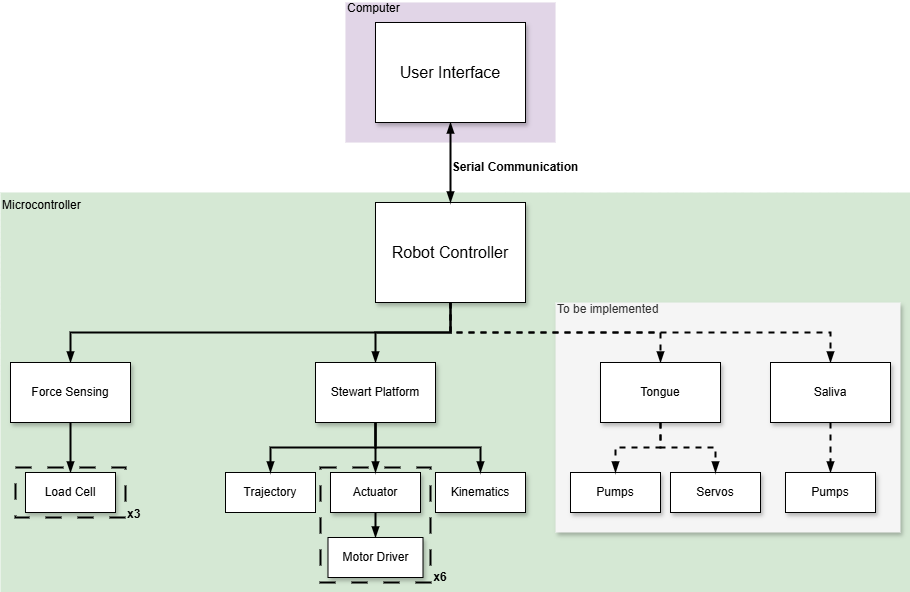
\includegraphics[width=\textwidth]{figures/code_structure.drawio.png}
\caption{Overall code structure.}
\label{fig:code_structure}
\end{figure}


\begin{figure}[H]
\centering
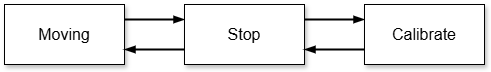
\includegraphics[width=0.6\textwidth]{figures/state_machine.drawio.png}
\caption{Robot controller state machine.}
\label{fig:state_machine}
\end{figure}

\subsubsection{Position control}

The Stewart Platform follows a 3D trajectory (x, y, z, roll, pitch, yaw) from a .csv file on the micro-SD card.
See section \ref{sec:motion-capture} for details on the recording protocol and data processing.
Each pose is defined by its position ${\bf t}=(x,y,z)$ and orientation given by the Euler angles $(\phi,\theta,\psi)$,
 which are the roll, pitch, and yaw angles respectively.
The trajectory is then linearly interpolated with a fixed time step chosen by the user.

\paragraph{Inverse kinematics}
For each pose in the trajectory, \texttt{Kinematics} computes the lengths of the six linear actuators that will achieve 
the desired pose of the platform, i.e. the inverse kinematics. To do so, we first compute the standard rotation matrix 
$R(\phi,\theta,\psi)$ for the Euler angles, which is defined as the product of three rotation matrices about 
the $Z$, $Y$, and $X$ axes:
\[
R(\phi,\theta,\psi) = R_Z(\psi) R_Y(\theta) R_X(\phi) =
\begin{pmatrix}
\cos\psi & -\sin\psi & 0 \\
\sin\psi & \cos\psi & 0 \\
0 & 0 & 1
\end{pmatrix}
\begin{pmatrix}
\cos\theta & 0 & \sin\theta \\
0 & 1 & 0 \\
-\sin\theta & 0 & \cos\theta
\end{pmatrix}
\begin{pmatrix}
1 & 0 & 0 \\
0 & \cos\phi & -\sin\phi \\
0 & \sin\phi & \cos\phi
\end{pmatrix}
\]

The platform joints ${\bf p}_i$, $i$ being the actuator index, are then rotated about a fixed point ${\bf c}$, 
which is the front of the gnathion, and translated by the user-defined home position ${\bf t}=(x,y,z)$, 
resulting in the world coordinates of the platform joints:
\[
{\bf w}_i = R\bigl({\bf p}_i-{\bf c}\bigr)+{\bf c}+{\bf t}.
\]

Finally, the actuator length is the Euclidean distance to the fixed base joint ${\bf b}_i$:
\[
\ell_i = \lVert {\bf w}_i-{\bf b}_i\rVert_2.
\]

\paragraph{PI controller}
For each actuator, its desired length is sent to a PI position controller, see Figure~\ref{fig:actuator_pi}.
To minimize the noise of the potentiometer feedback, we apply a low-pass filter averaging the last 10 samples.
\begin{figure}[H]
\centering
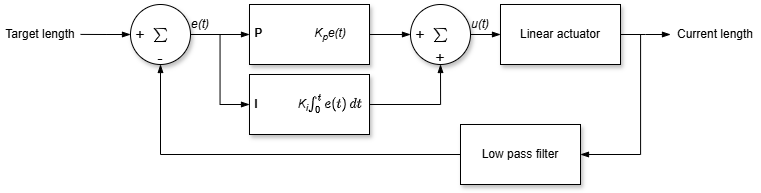
\includegraphics[width=\textwidth]{figures/actuator_pi.drawio.png}
\caption{Position PI controller for the linear actuators.}
\label{fig:actuator_pi}
\end{figure}

\subsection{Data acquisition and processing}
\label{sec:motion-capture}

\paragraph{Subjects.} 
Two healthy adult volunteers (author and project supervisor) participated in this pilot recording. Owing to time constraints and the exploratory 
nature of the study, no additional subjects were recruited.

\paragraph{Motion-capture acquisition.}
Mandibular motion was recorded with a five-camera OptiTrack system sampling at 120 Hz.
Four reflective markers arranged in a square were attached to the forehead and served as a head-fixed reference frame.
A second set of three markers forming a triangle was placed on the gnathion.
Two additional lip markers were recorded but later discarded because a single marker cannot encode orientation. \cite{motion_capture_adult,motion_capture_children}

The subject then performed the motion sequences listed in Table~\ref{tab:recording-protocol}. Each frame was saved by Motive as a \texttt{.csv} file that contains
the 3-D marker positions (in millimetres) and the orientation of each marker set as quaternions. The calibrated volume had a residual error of $0.3\,$mm.
% TODO: insert a photograph of the marker placement

\begin{table}[H]
  \centering
  \small                                   
  \renewcommand{\arraystretch}{1.1}  
  \begin{tabularx}{\textwidth}{@{} c l l @{}}      
    \toprule
    \textbf{Food} & \textbf{Motion} & \textbf{\textit{Optional:} Duration} \\
    \midrule
    % ---------- Empty mouth block ----------
    Empty mouth & 20$\times$ open–close cycles                 & —     \\[1pt]
    \midrule
    % ---------- Chewing-gum block ----------
    \multirow{5}{*}{\parbox[c]{3.2cm}{\centering Chewing gum\\(Xylit-Pro,\\\emph{Excitemint})}}
      & Random side chewing                                    & 2 min \\[1pt]
      & Right-side chewing                                     & 1 min \\[1pt]
      & Left-side chewing                                      & 1 min \\[1pt]
      & Front-teeth-only chewing                               & 1 min \\ 
    \midrule
    % ---------- Biscuit block ----------
    \multirow{5}{*}{\parbox[c]{3.2cm}{\centering Biscuits\\(Bretzeli, \emph{Kambli})}}
      & random chewing                                    & — \\[1pt]
      & front-teeth chew → right-side chew                & — \\[1pt]
      & front-teeth chew → left-side chew                  & — \\[1pt]
      & \textit{fast} random chewing                      & — \\[1pt]
      & \textit{slow} random chewing                       & — \\
    \bottomrule
  \end{tabularx}
  \caption{Recording protocol. \textit{Notes:}  
  For chewing-gum trials the first run began with an unchewed piece and the same gum was kept for all subsequent motions.  
  For biscuit trials each run started with an empty, closed mouth; the subject then placed a biscuit, chewed as instructed, and swallowed.}
  \label{tab:recording-protocol}
\end{table}

\paragraph{Data processing.}
To reduce the noise, we apply a 4th-order butterworth filter to the data. The cutoff frequency is set to 6Hz, as human mastication frequency is around 1Hz to 2Hz %\cite{chewing_frequency} TODO: find paper
. \\
The data is then transformed to the head reference frame using rotation matrices. 








\section{Results}
\subsection{Motion captured chewing trajectories}
\label{sec:traj_result}

Figures~\ref{fig:trajectory_plot} shows a trajectory obtained using from Section~\ref{sec:motion-capture}. The vertical displacement clearly reveals cyclic jaw movements, 
identifiable by recurring peaks that correspond to the opening and closing 
phases of the chewing cycle. The horizontal components (x and y) show a pattern consistent with reported human data \cite{chewing_traj}.

The orientation data on the other hand is less reliable as no clear pattern can be seen throughout the trajectory. Several factors described in Section~\ref{sec:motion_capture_limitations} 
may contribute to this inaccuracy. 

Nonetheless, the trajectory remains sufficiently accurate to evaluate the robot's position control performance and serves as a useful initial 
benchmark.

% \begin{figure}[H]
% \centering
% \begin{minipage}{.45\textwidth}
%   \centering
%   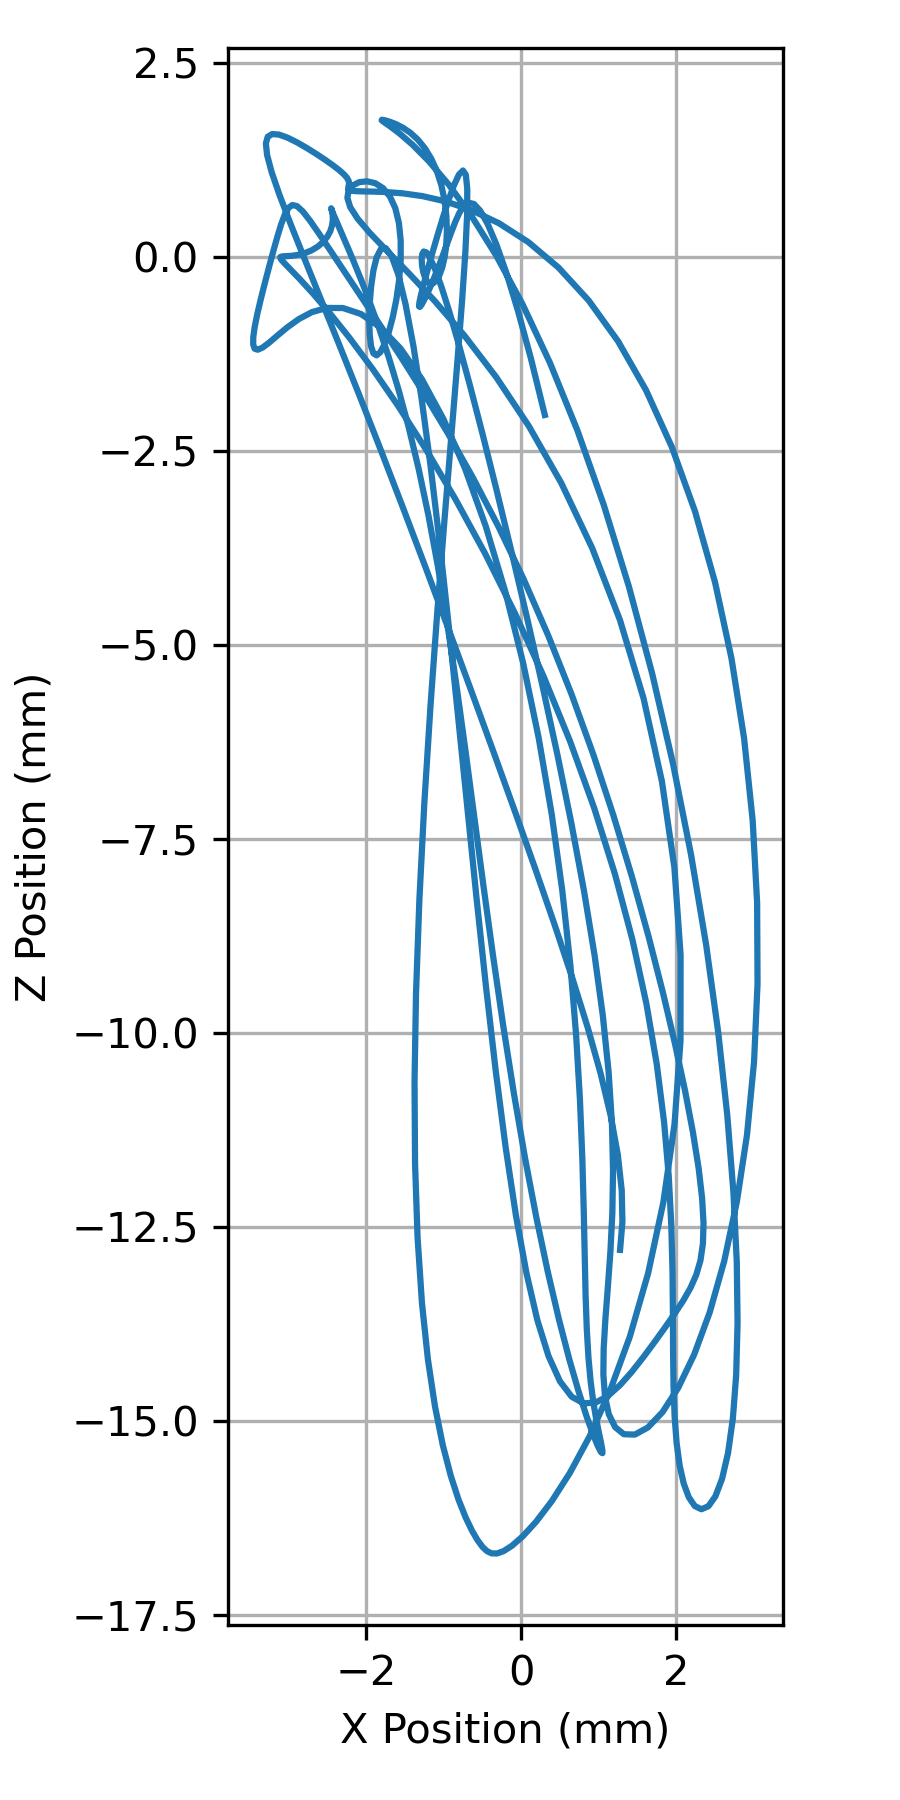
\includegraphics[height=6cm]{figures/x_vs_z_position.png}
%   \subcaption{}
%   \label{fig:x-z}
% \end{minipage}
% \begin{minipage}{.45\textwidth}
%   \centering
%   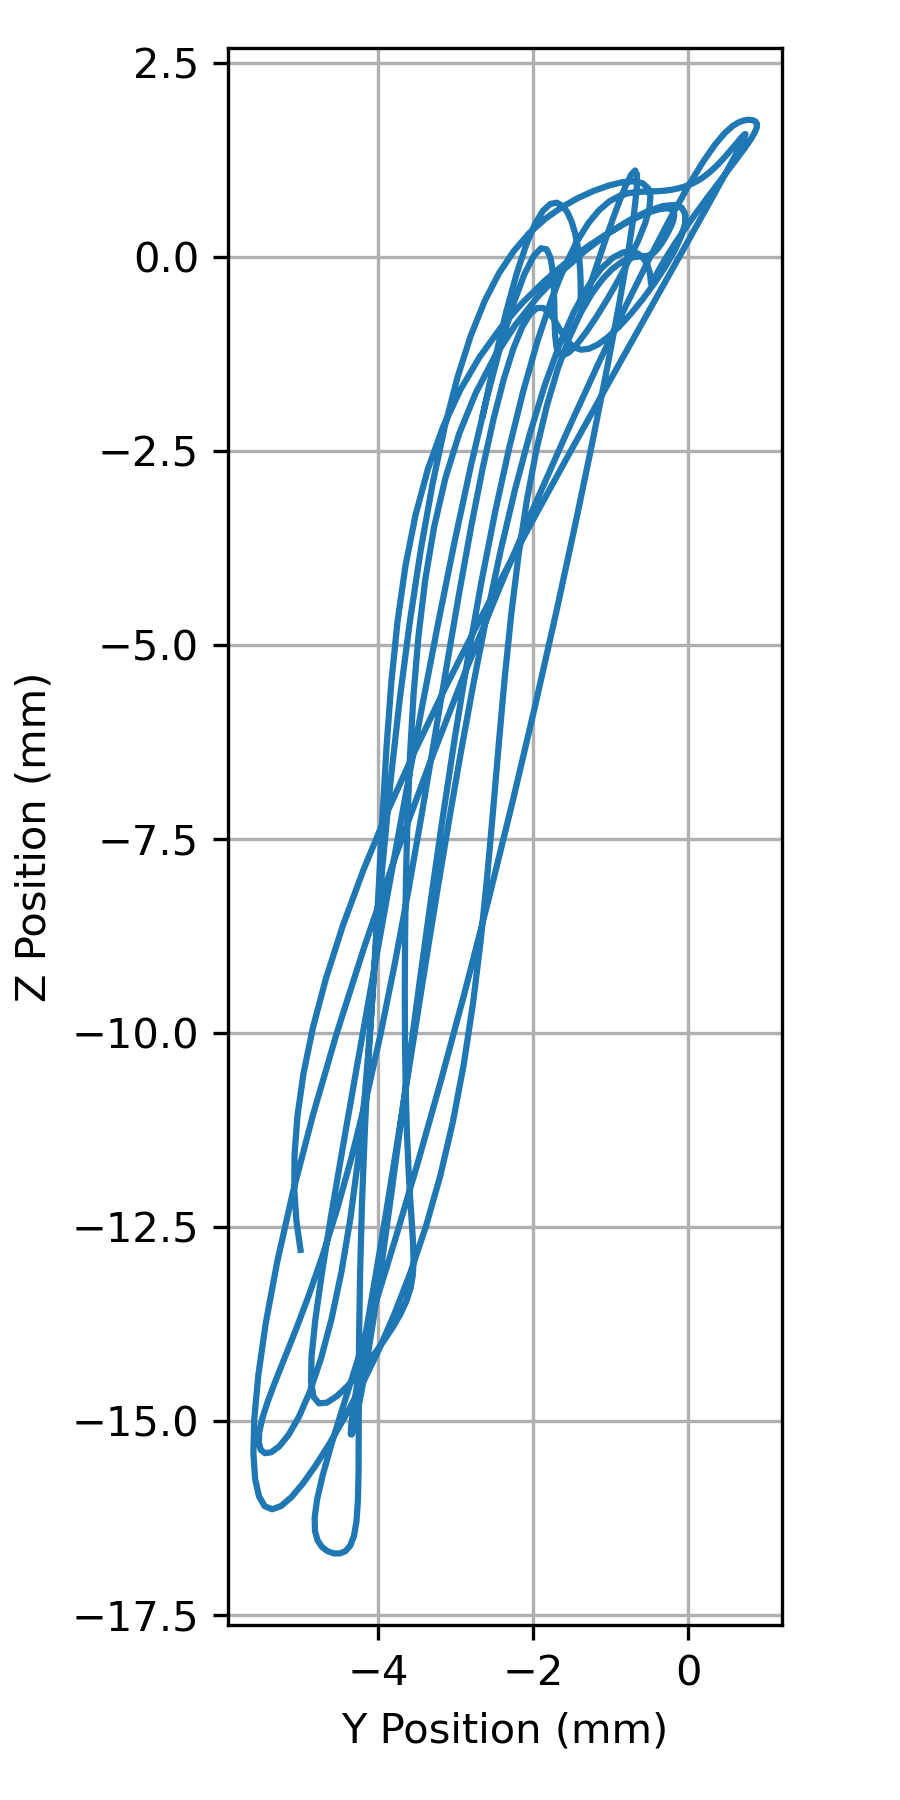
\includegraphics[height=6cm]{figures/y_vs_z_position.png}
%   \subcaption{}
%   \label{fig:y-z}
% \end{minipage}
% \caption{Position of the jaw in the x-z plane (a) and y-z plane (b).}
% \label{fig:xy-z}
% \end{figure}

\begin{figure}[H]
    \centering
    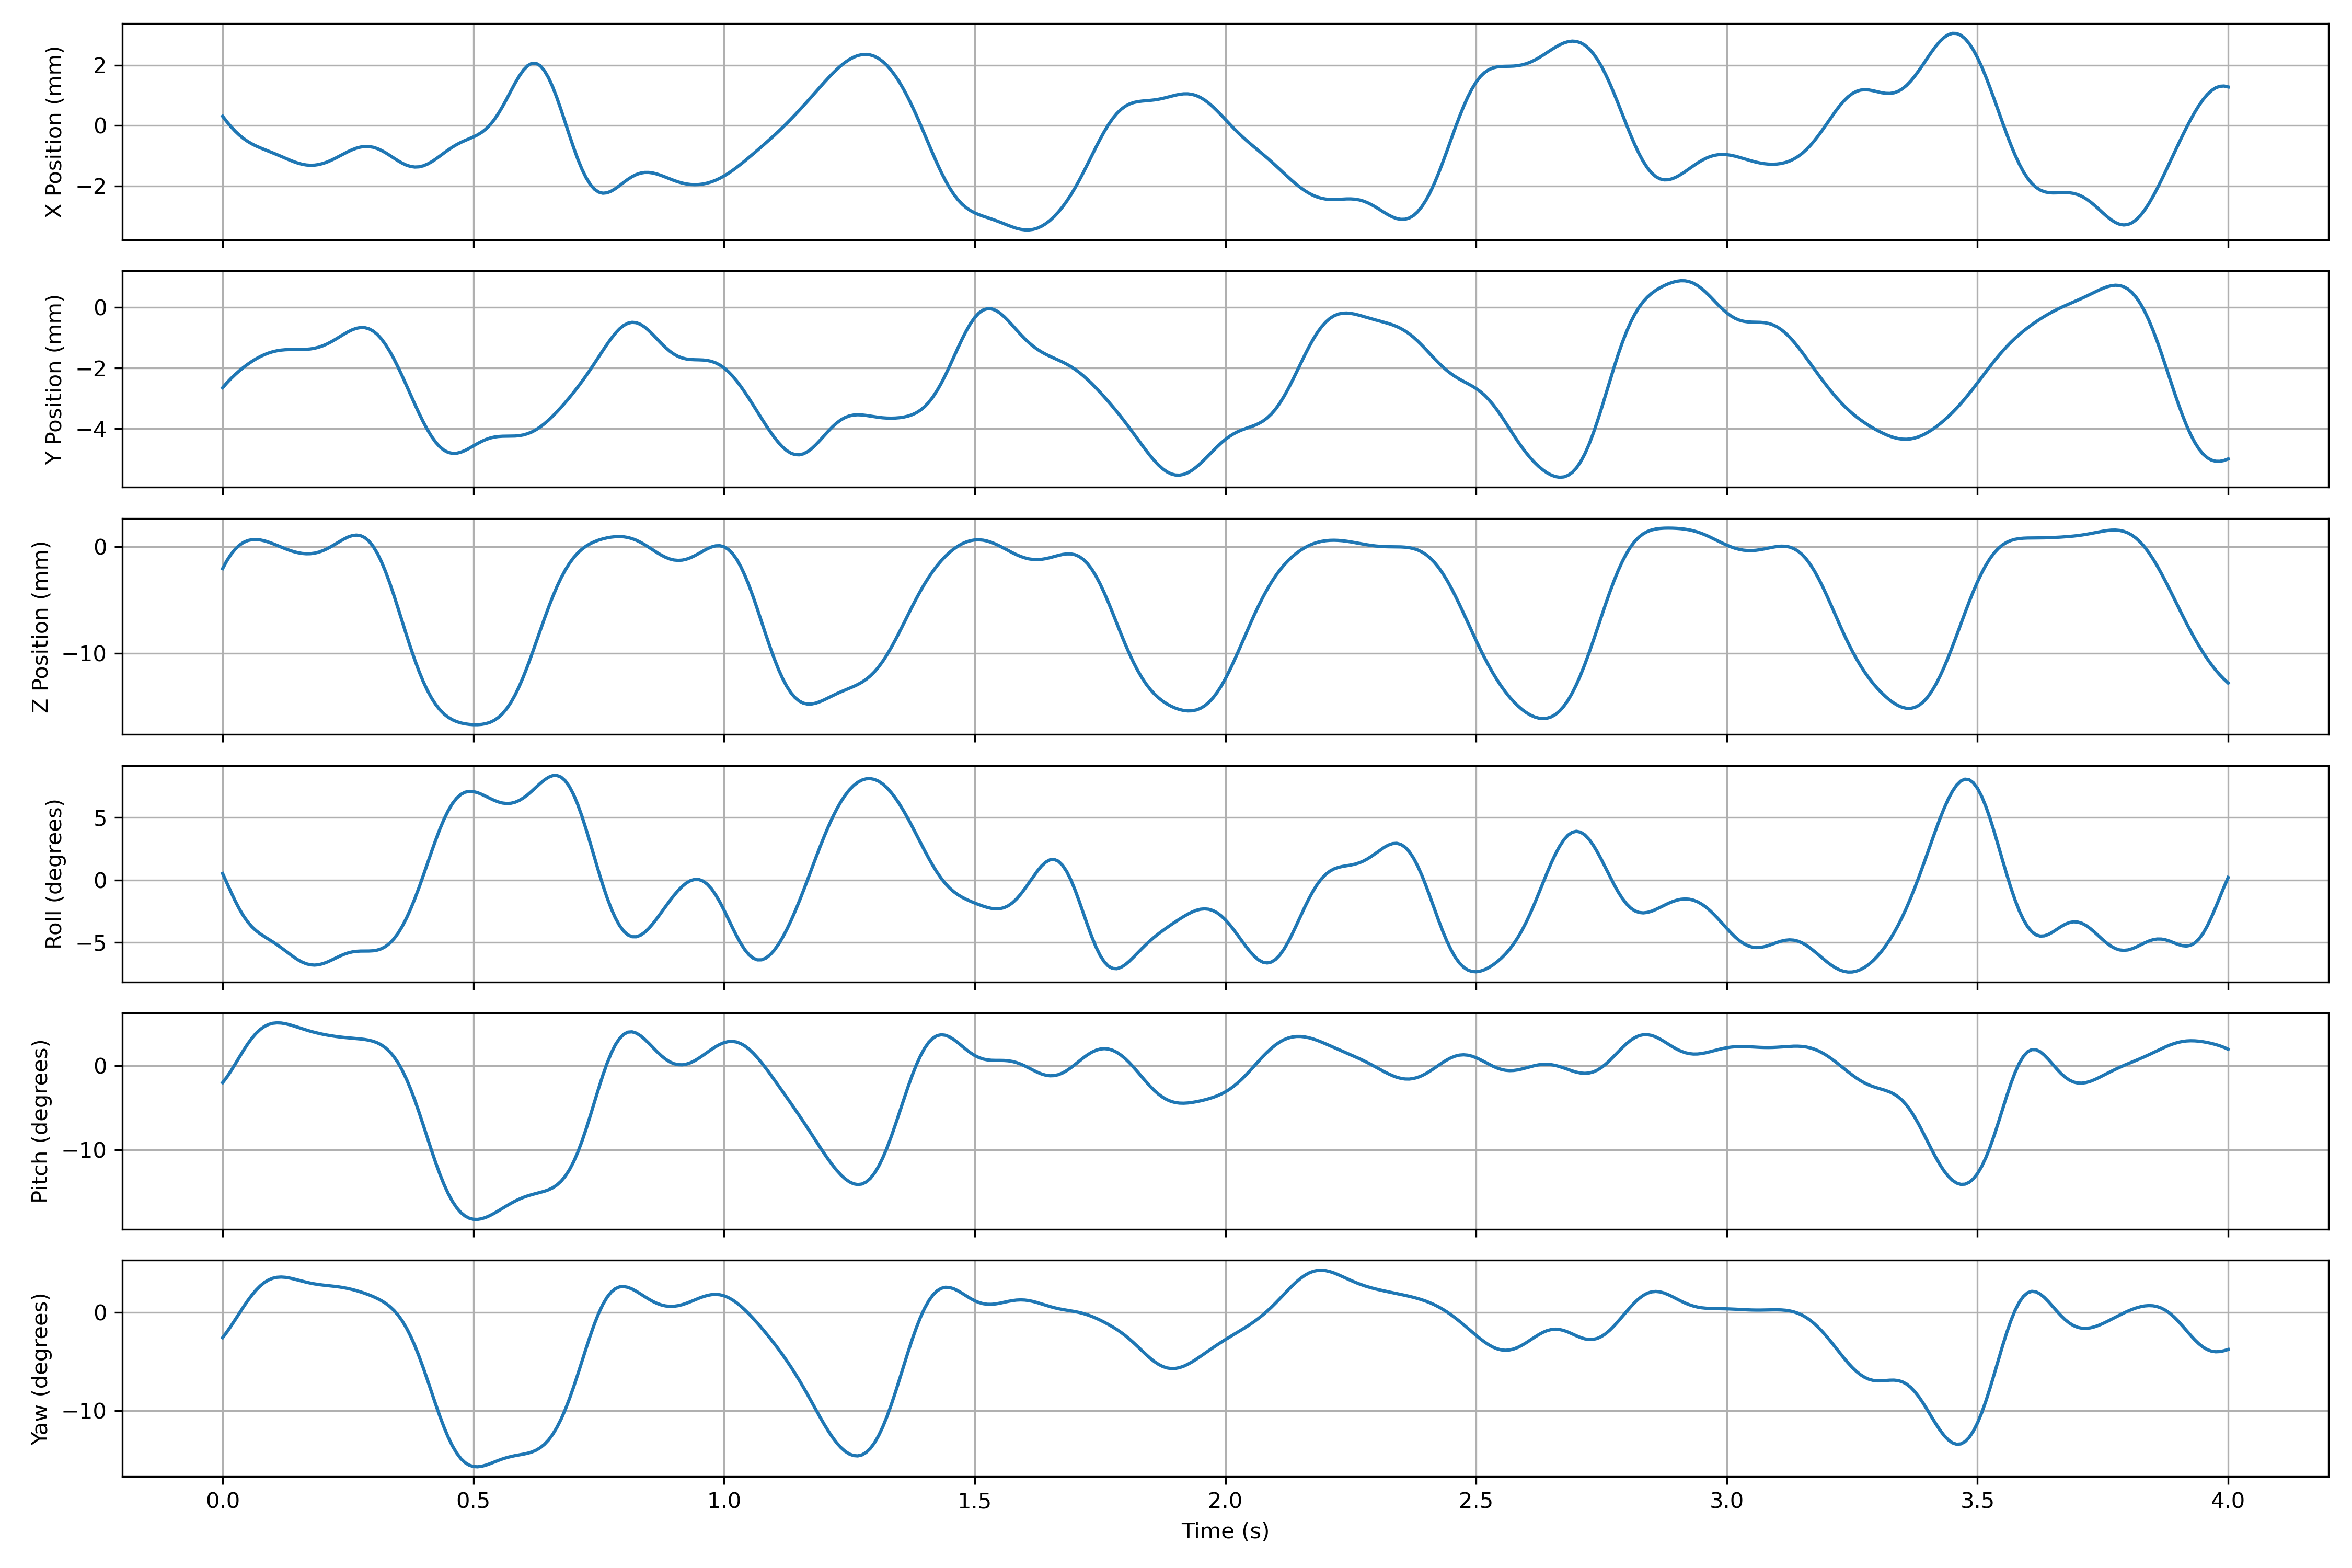
\includegraphics[width=\textwidth]{figures/trajectory_plot.png}
    \caption{Random side chewing gum mastication trajectory.}
    \label{fig:trajectory_plot}
\end{figure}

\subsection{Position control}

\paragraph{Speed and accuracy}
To evaluate the performance of the position control system, we investigated the robot's ability to track a predefined trajectory at varying speeds. 
In this context, “speed” refers to the time interval between consecutive trajectory points. While the motion capture data was recorded at 120 Hz 
(approximately every 8.3 ms), the playback was tested at longer intervals: 40 ms (25 Hz), 50 ms (20 Hz), 60 ms (16.67 Hz), 70 ms (14.29 Hz), 80 ms 
(12.5 Hz), 90 ms (11.11 Hz), and 100 ms (10 Hz).

For this test, a 10-second segment of chewing motion was used. Figure~\ref{fig:actuator_delays_2} illustrates the tracking performance of actuator 2 
at the various speeds. To quantify timing discrepancies, we conducted a cross-correlation analysis between the target and actual actuator lengths, 
providing both time delays (Figure~\ref{fig:actuator_delays_2}) and cross-correlation coefficients (Figure~\ref{fig:actuator_rhos_2}).

The results show that at a sampling interval of 100 ms (10 Hz), the robot tracks the trajectory well, with an average delay of ~0.7 s and 
cross-correlation coefficients exceeding 0.975. However, performance degrades significantly at higher speeds (i.e., shorter intervals), 
as reflected in both increased delays and a drop in correlation values—especially below 80 ms, where the tracking error becomes pronounced 
and key trajectory peaks are missed.

\begin{figure}[H]
    \centering
    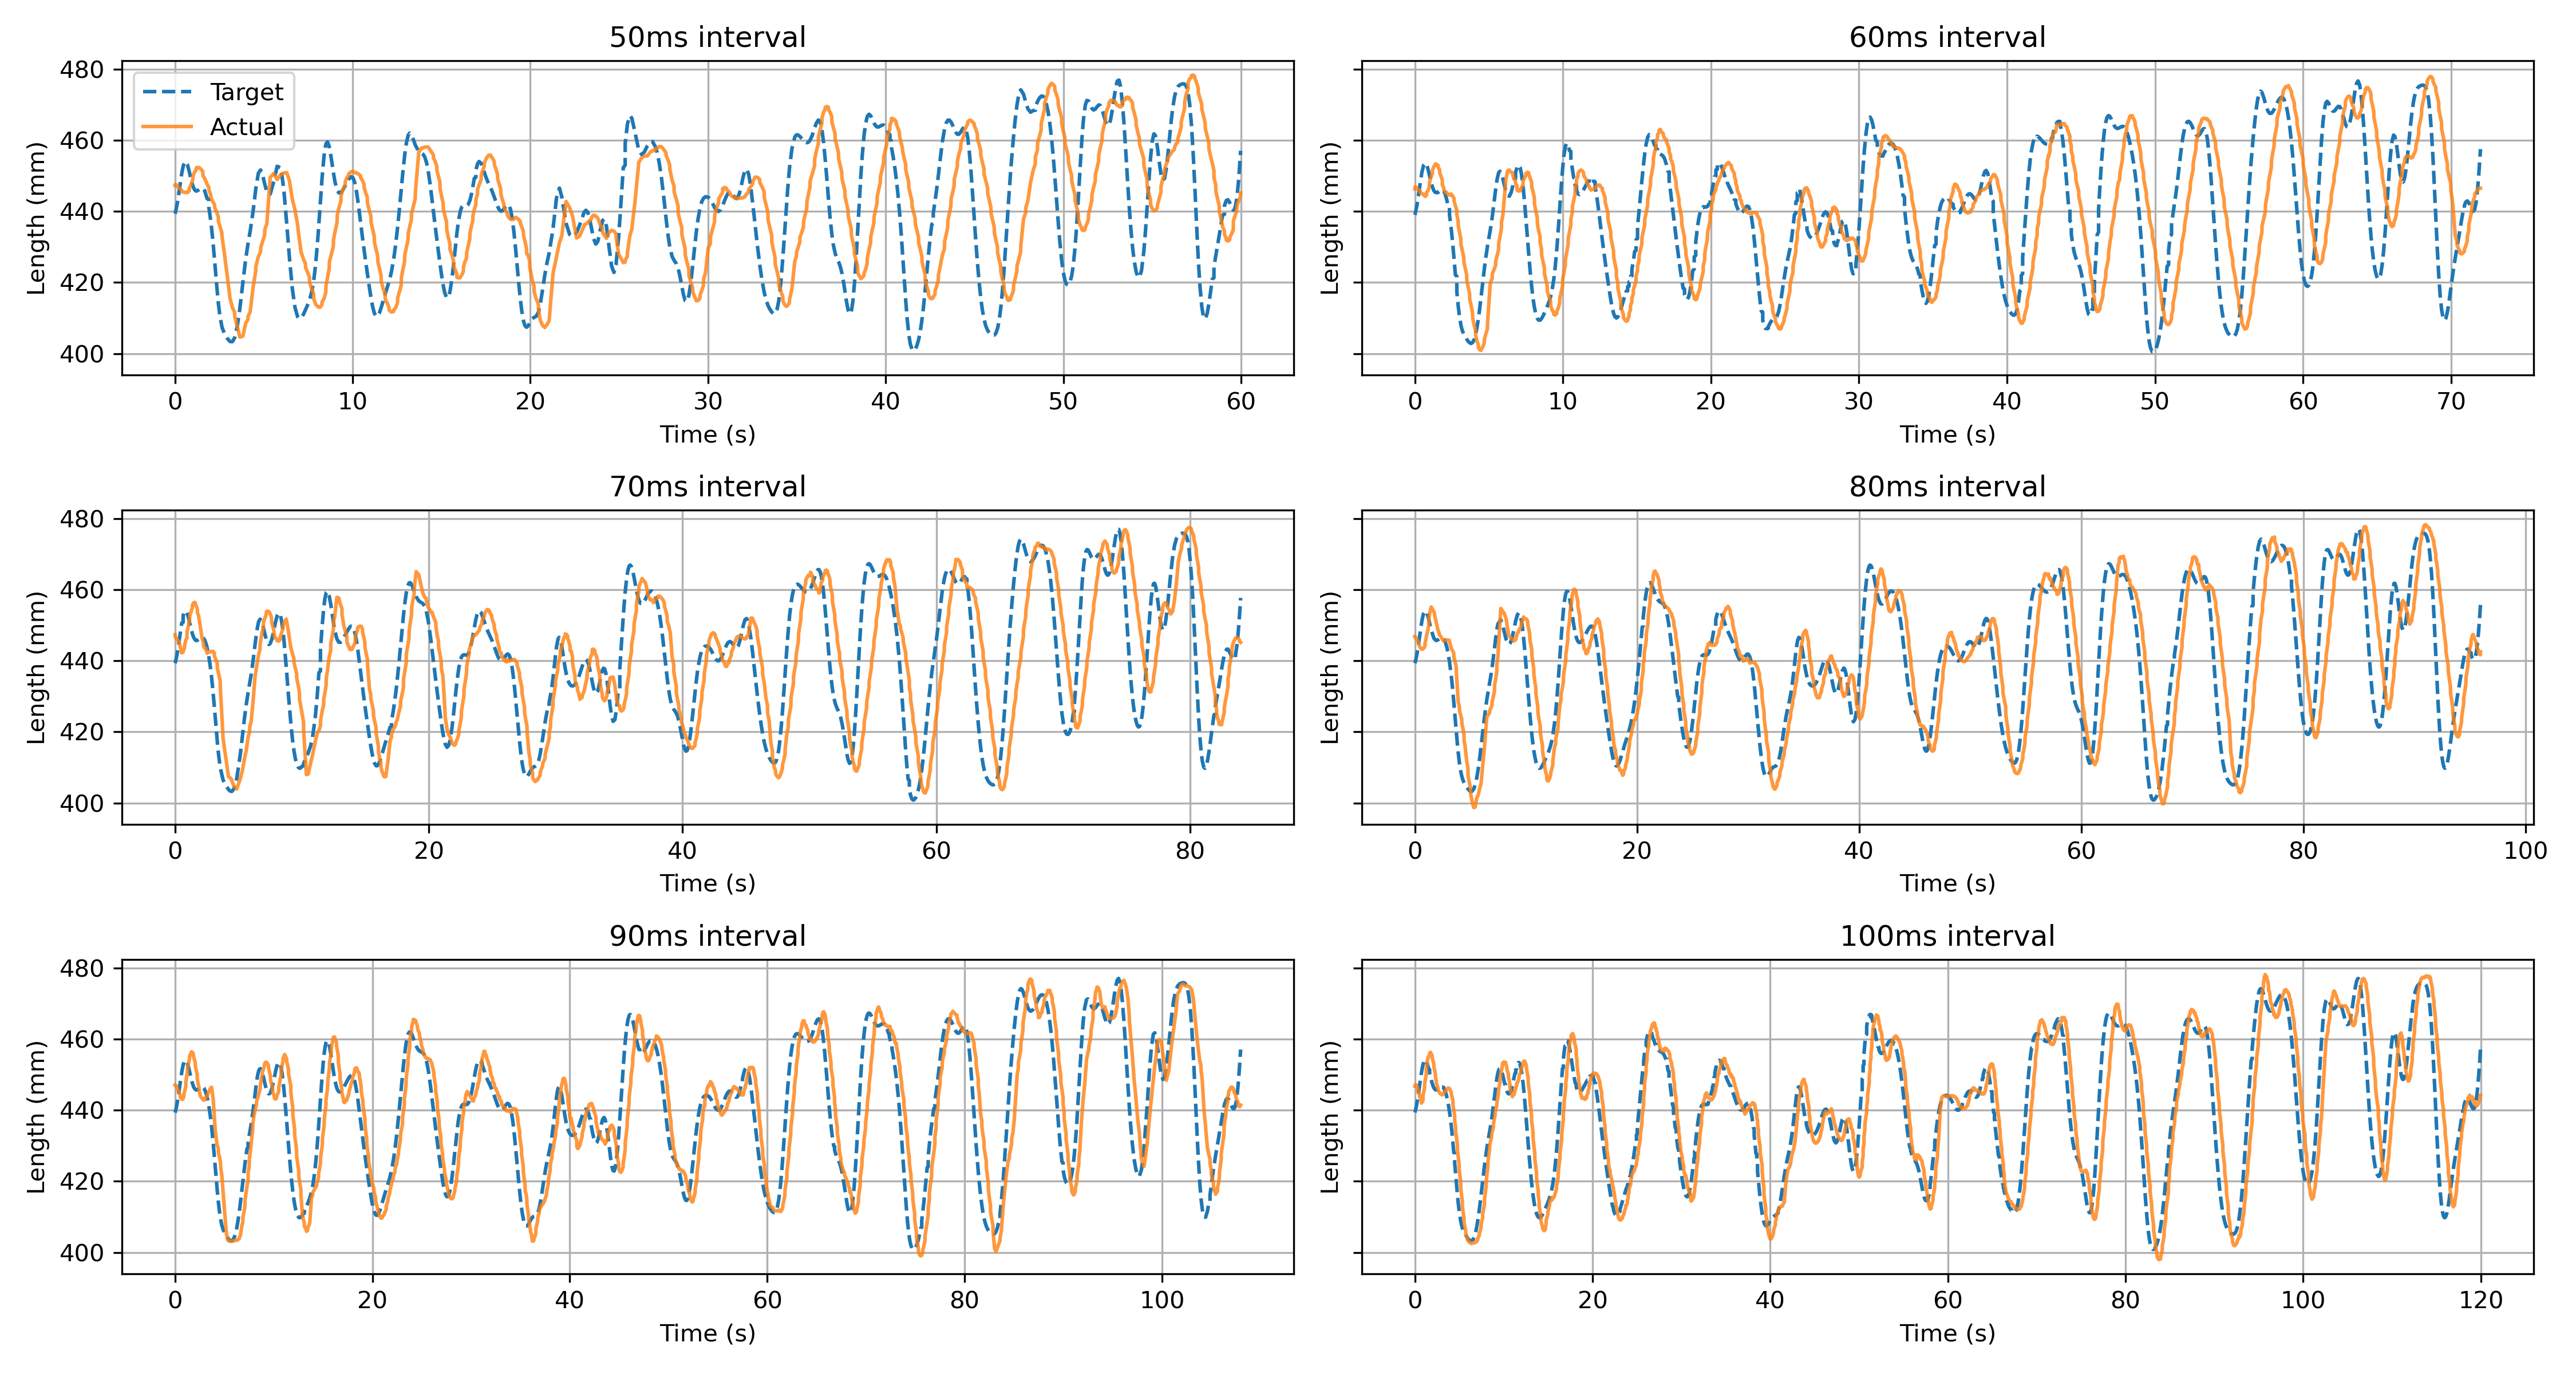
\includegraphics[width=\textwidth]{figures/actuator_2_trajectories.png}
    \caption{Performance of position control of actuator 2 across different time intervals between trajectory points.}
    \label{fig:position_control}
\end{figure}

\begin{figure}[H]
    \centering
    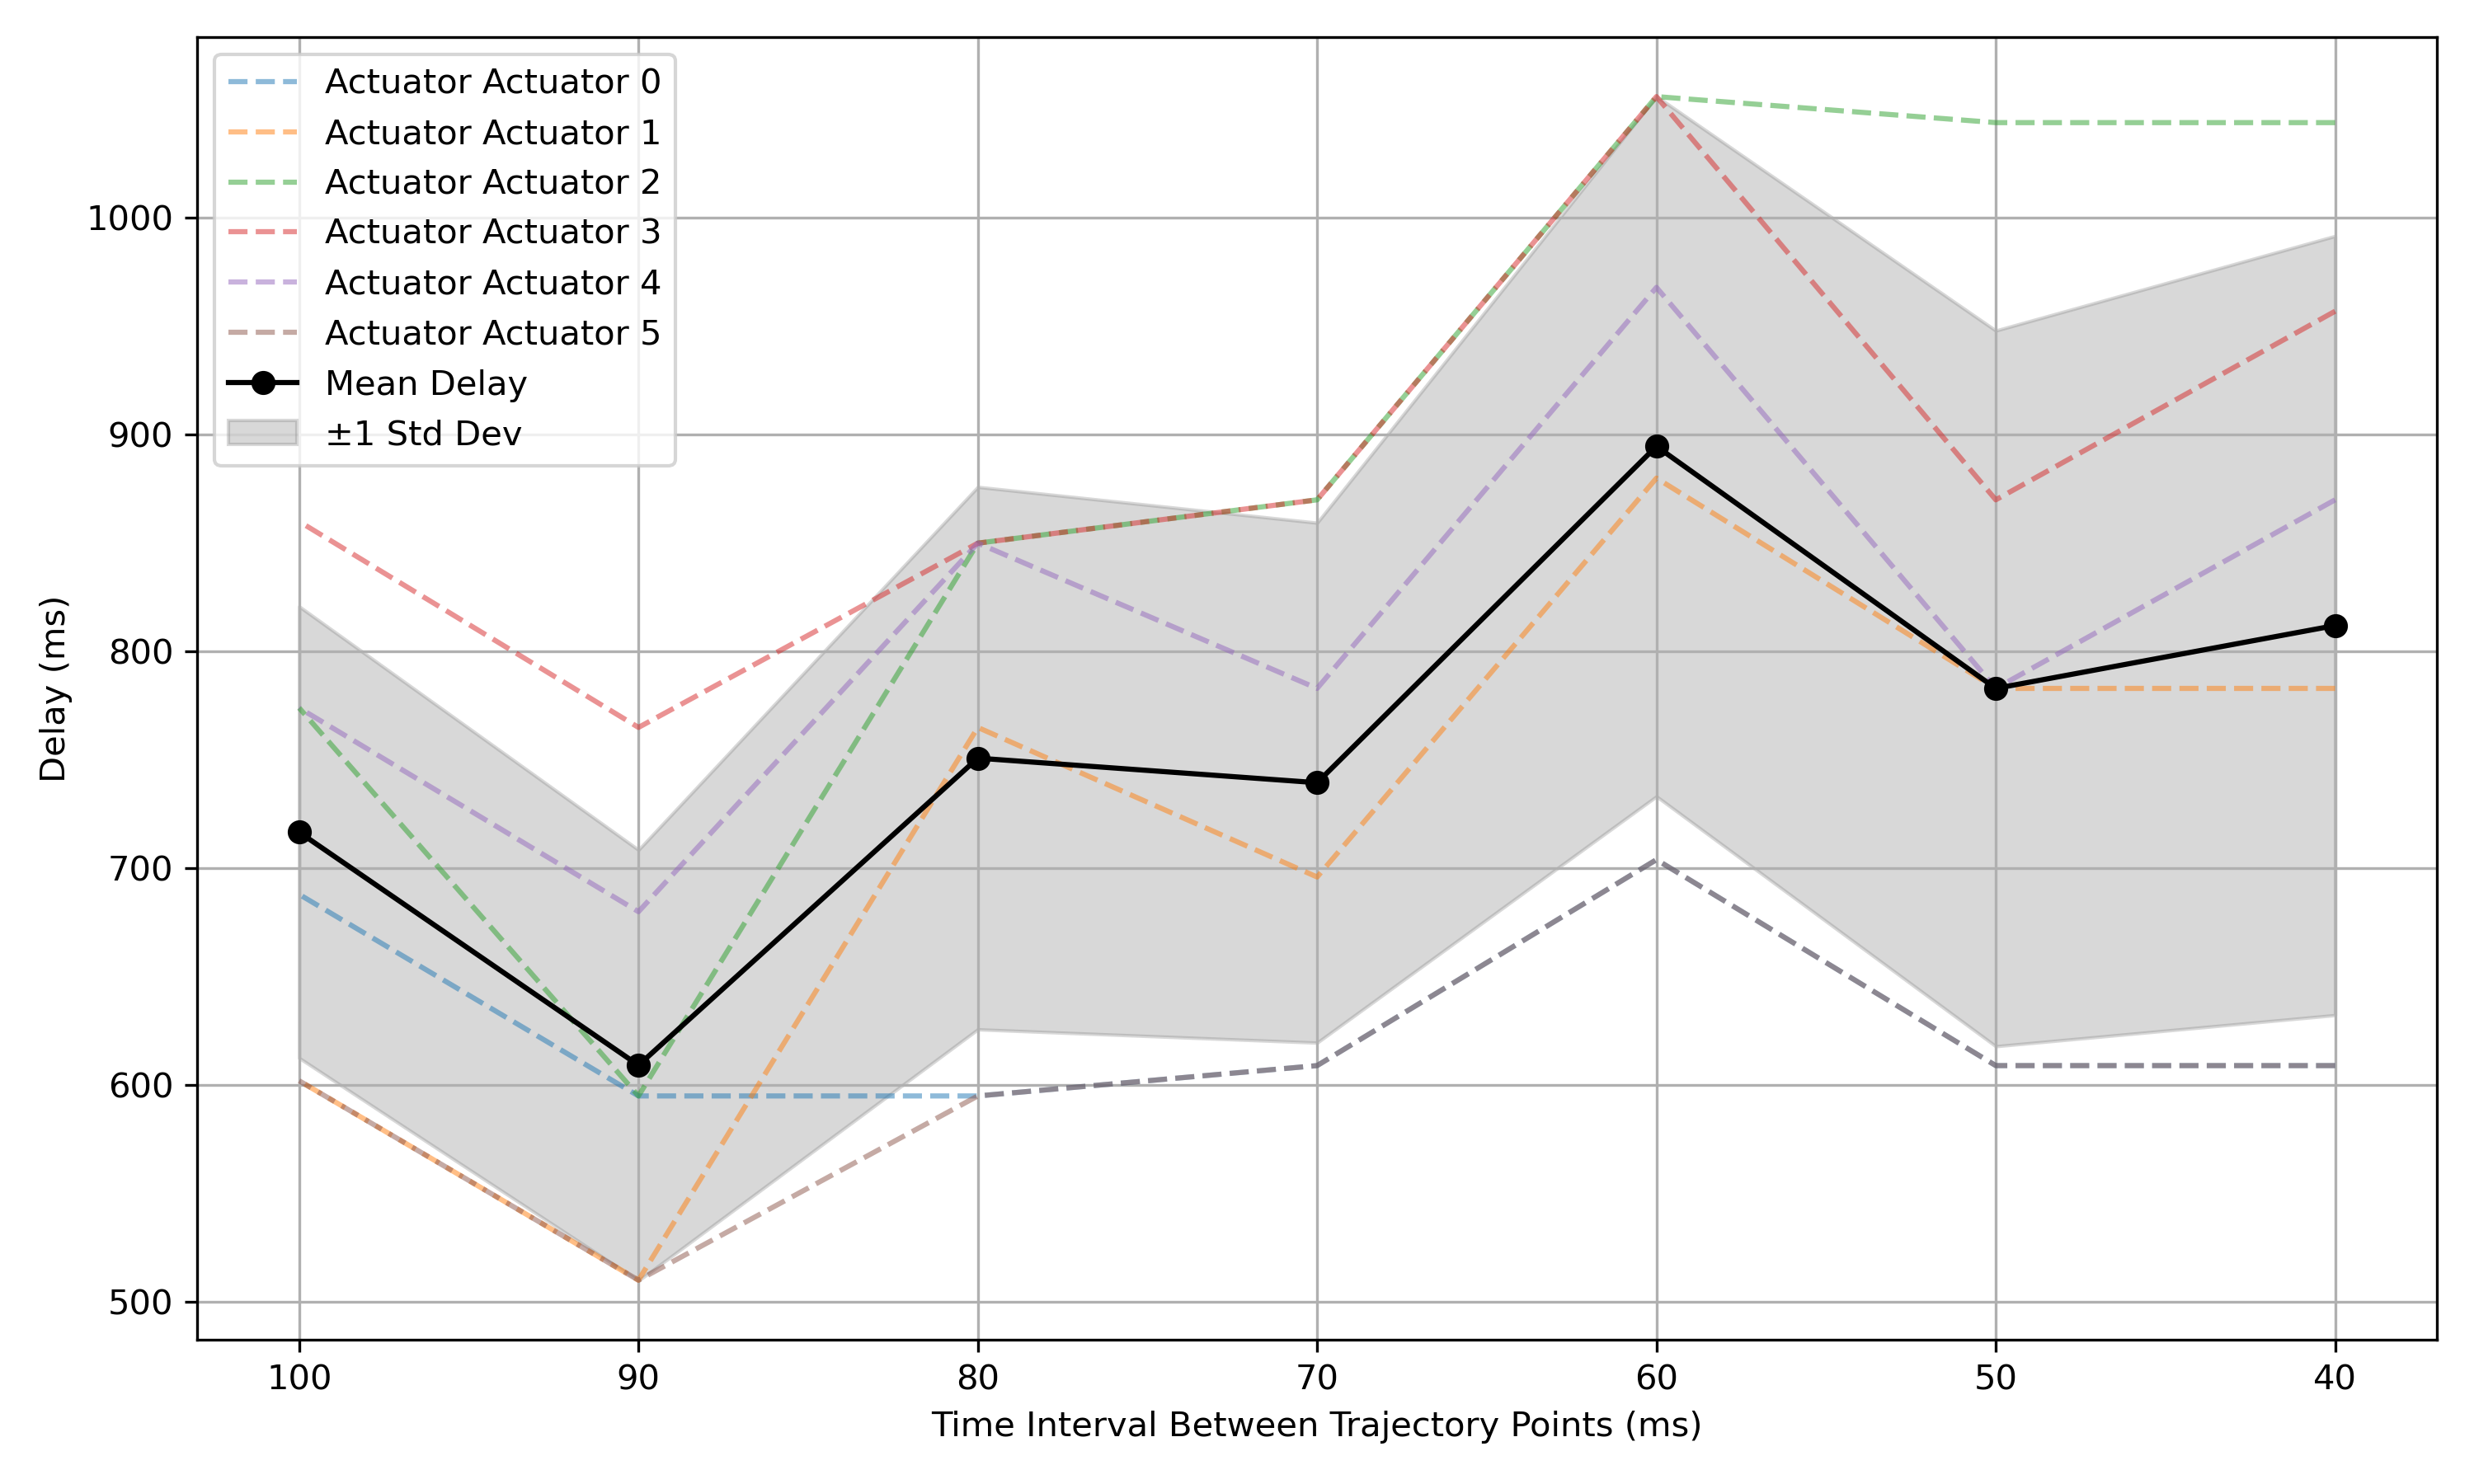
\includegraphics[width=0.6\textwidth]{figures/actuator_delays.png}
    \caption{Delays between target and actual actuator length across different time intervals.}
    \label{fig:actuator_delays_2}
\end{figure}

\begin{figure}[H]
    \centering
    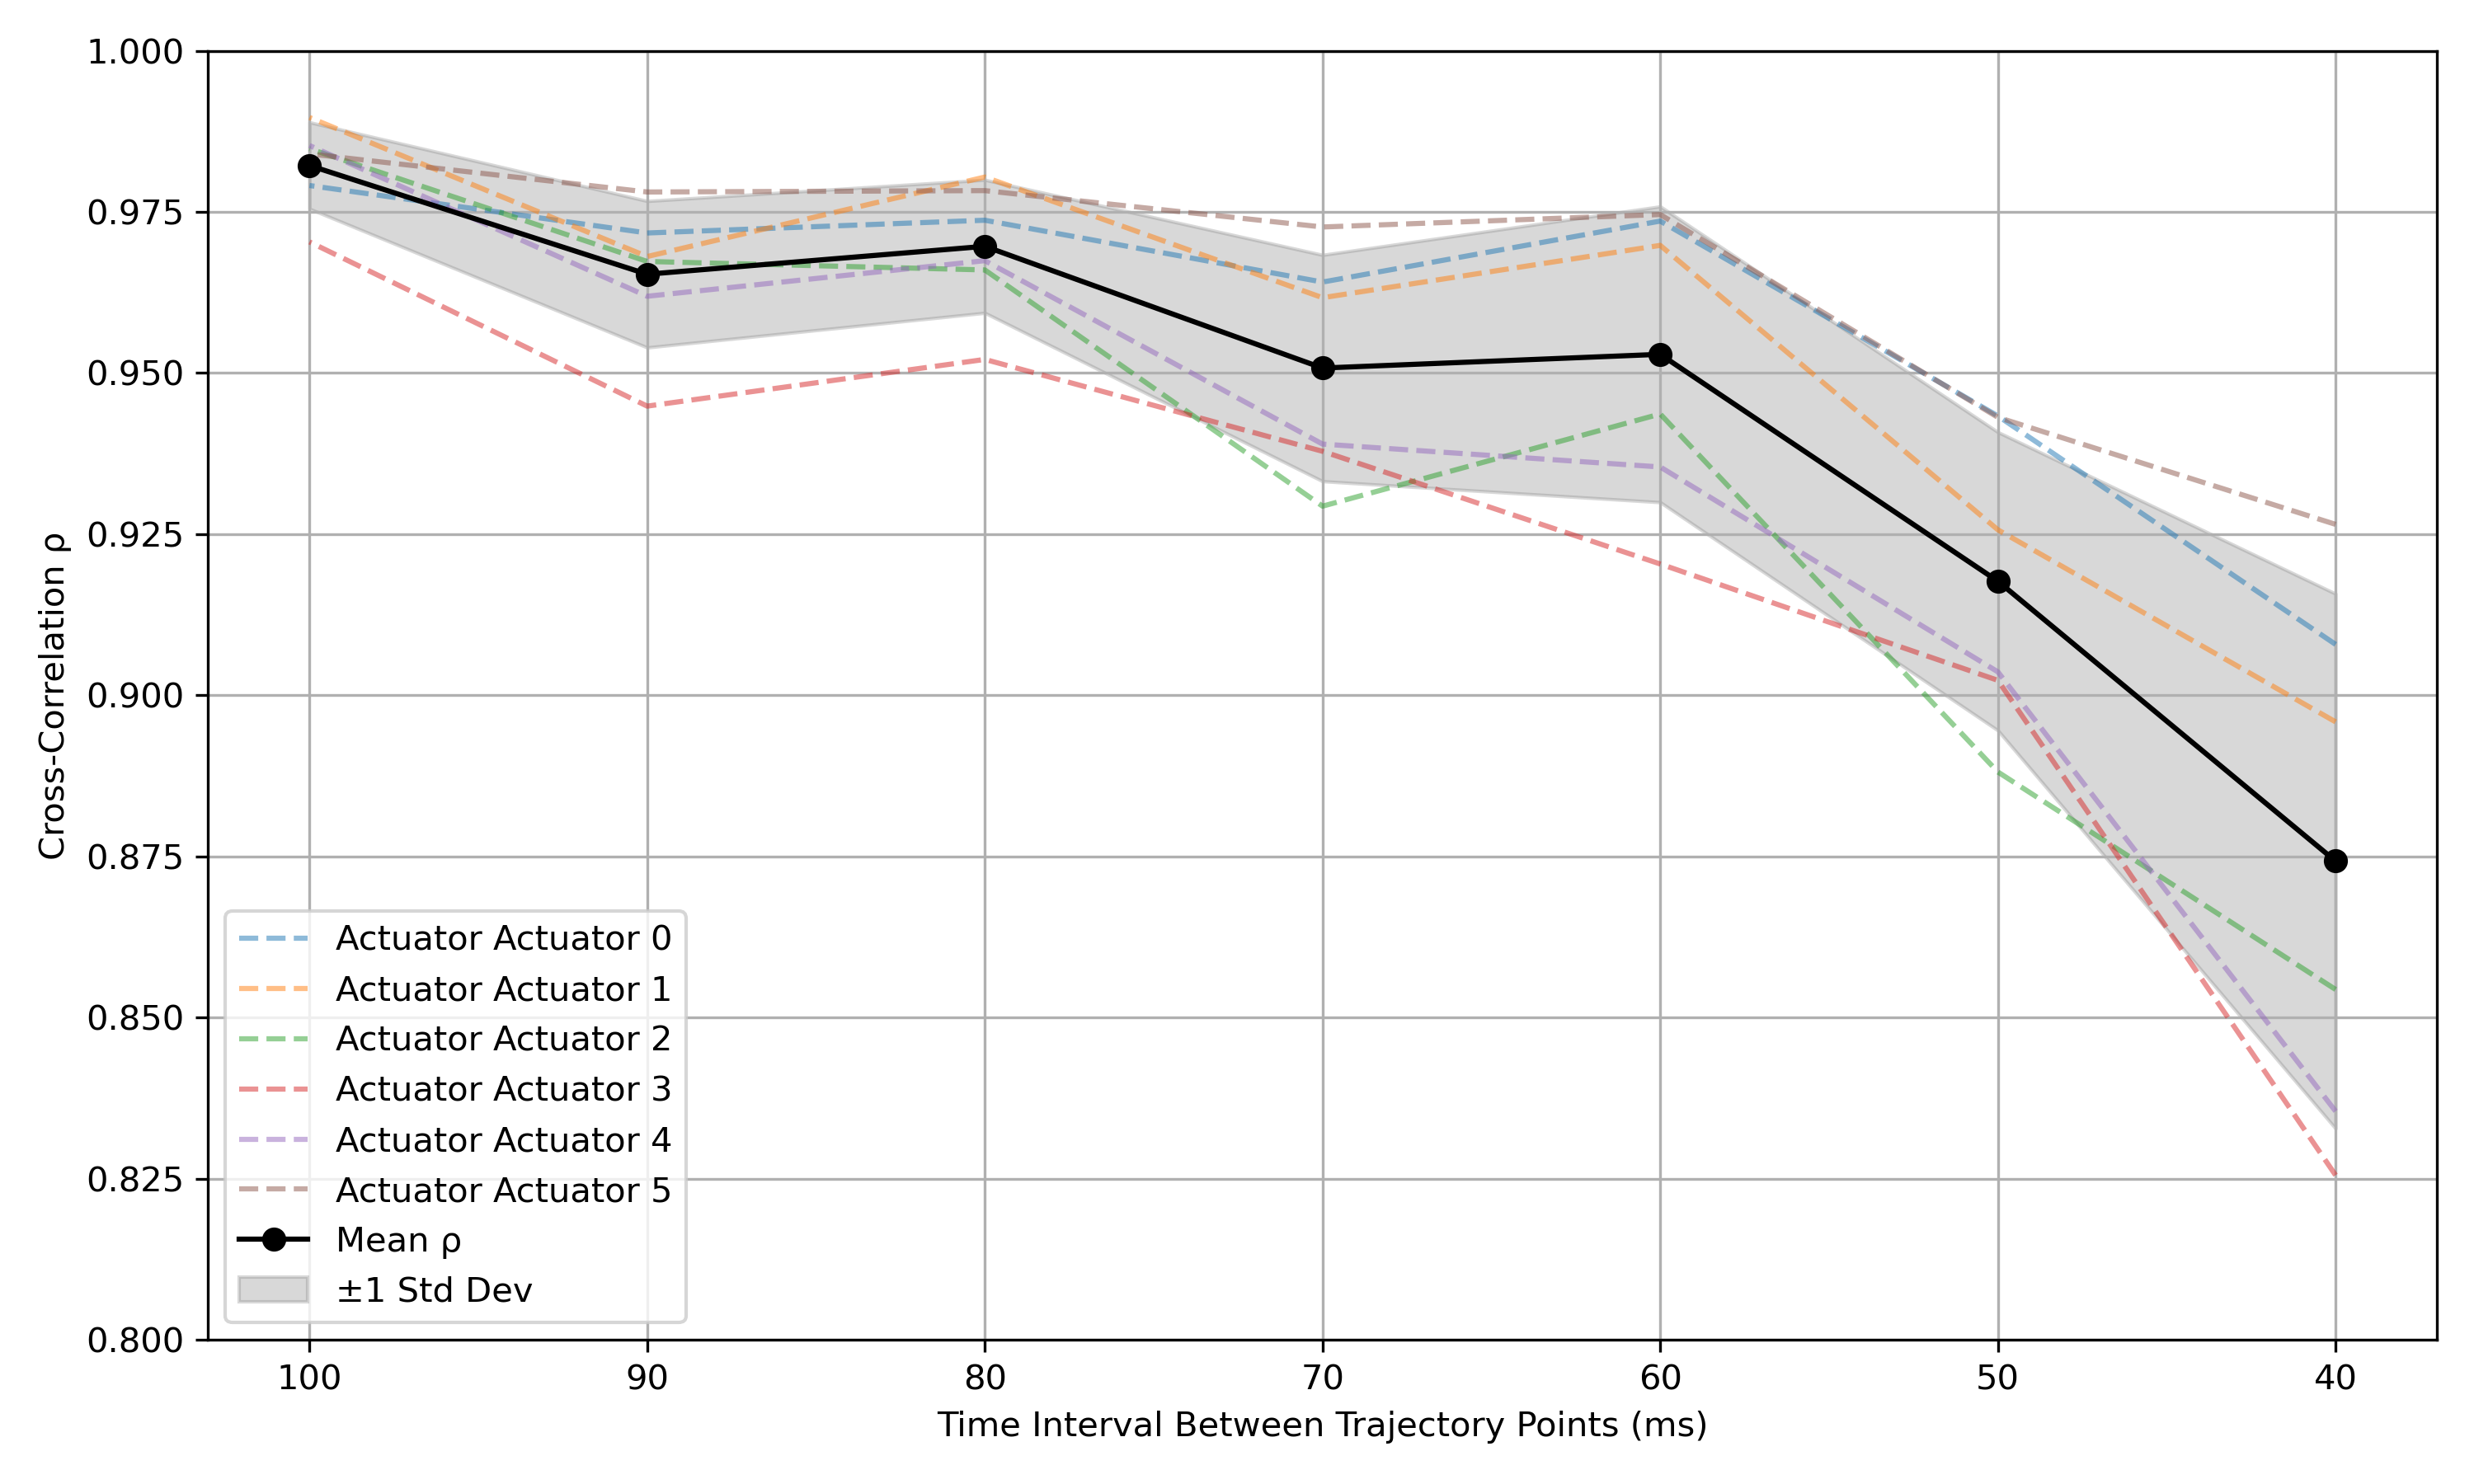
\includegraphics[width=0.6\textwidth]{figures/actuator_rhos.png}
    \caption{Cross-correlation coefficients across actuators for different time intervals.}
    \label{fig:actuator_rhos_2}
\end{figure}

\subsection{Force analysis}

\subsubsection{Maximum force}

The robot's vertical force generation capabilities were assessed using manual control mode normally used to set the robot's home position during calibration. 
The platform was driven at its highest height under active force feedback while avoiding structural failure. The upper bound of the robot's vertical force 
output was constrained by the stiffness of the upper jaw structure, which visibly bent under high vertical force. Table~\ref{tab:max_force} shows the 
maximum forces recorded by the three load cells during this test, see Figure~\ref{fig:load_cells_axis}.
for the load cell positions. The results shows that most of the vertical force is applied on the back load cells, which reflects the 
anatomical load pattern during full occlusion, where the molars bear the majority of chewing forces. Same for the antero-posterior force ($F_y$) where most of it 
is applied on the front load cell, i.e. the incisors. The total vertical, lateral and antero-posterior force output of the robot are well within the average 
forces during healthy human chewing \cite{shear_force}, although $F_z$ is below the maximum bit force from Table~\ref{tab:functional_criteria}.
\begin{table}[H]
    \centering
    \begin{tabular}{p{4cm} p{2cm} p{2cm} p{2cm}}
        \toprule
        \textbf{Load Cell} & \textbf{$F_{z,max}$ (N)} & \textbf{$F_{y,max}$ (N)} & \textbf{$F_{x,max}$ (N)} \\
        \midrule
        Back Right Load Cell & 124.63 & 59.64 & 123.85 \\
        Back Left Load Cell & 124.63 & 23.95 & 67.84  \\
        Front Load Cell & 66.28 & 81.38 & 123.07  \\
        \midrule
        \textbf{Total Force} & \textbf{315.98} & \textbf{103.08} & \textbf{125.71} \\
        \bottomrule       
    \end{tabular}
    \caption{Maximal forces recorded by the load cells during the force test.}
    \label{tab:max_force}
\end{table}

\subsubsection{Force feedback distribution}

To evaluate the spatial resolution of the force sensing system, we applied a simple vertical trajectory while placing a piece of gum-like material 
at three distinct positions between the teeth: back right, front, and back left. The vertical force output from each of the three load cells was 
recorded (Figure~\ref{fig:force_distribution_gum}).

The plot clearly shows three distinct peaks corresponding to the three test positions, confirming the system's capability to localize force application 
across the dental arch. Additionally, when force is applied at the back, the front load cell registers a smaller secondary response. This is consistent 
with the mechanical coupling in the mounting structure, as the front load cell is physically situated between the two rear ones.

\begin{figure}[H]
    \centering 
    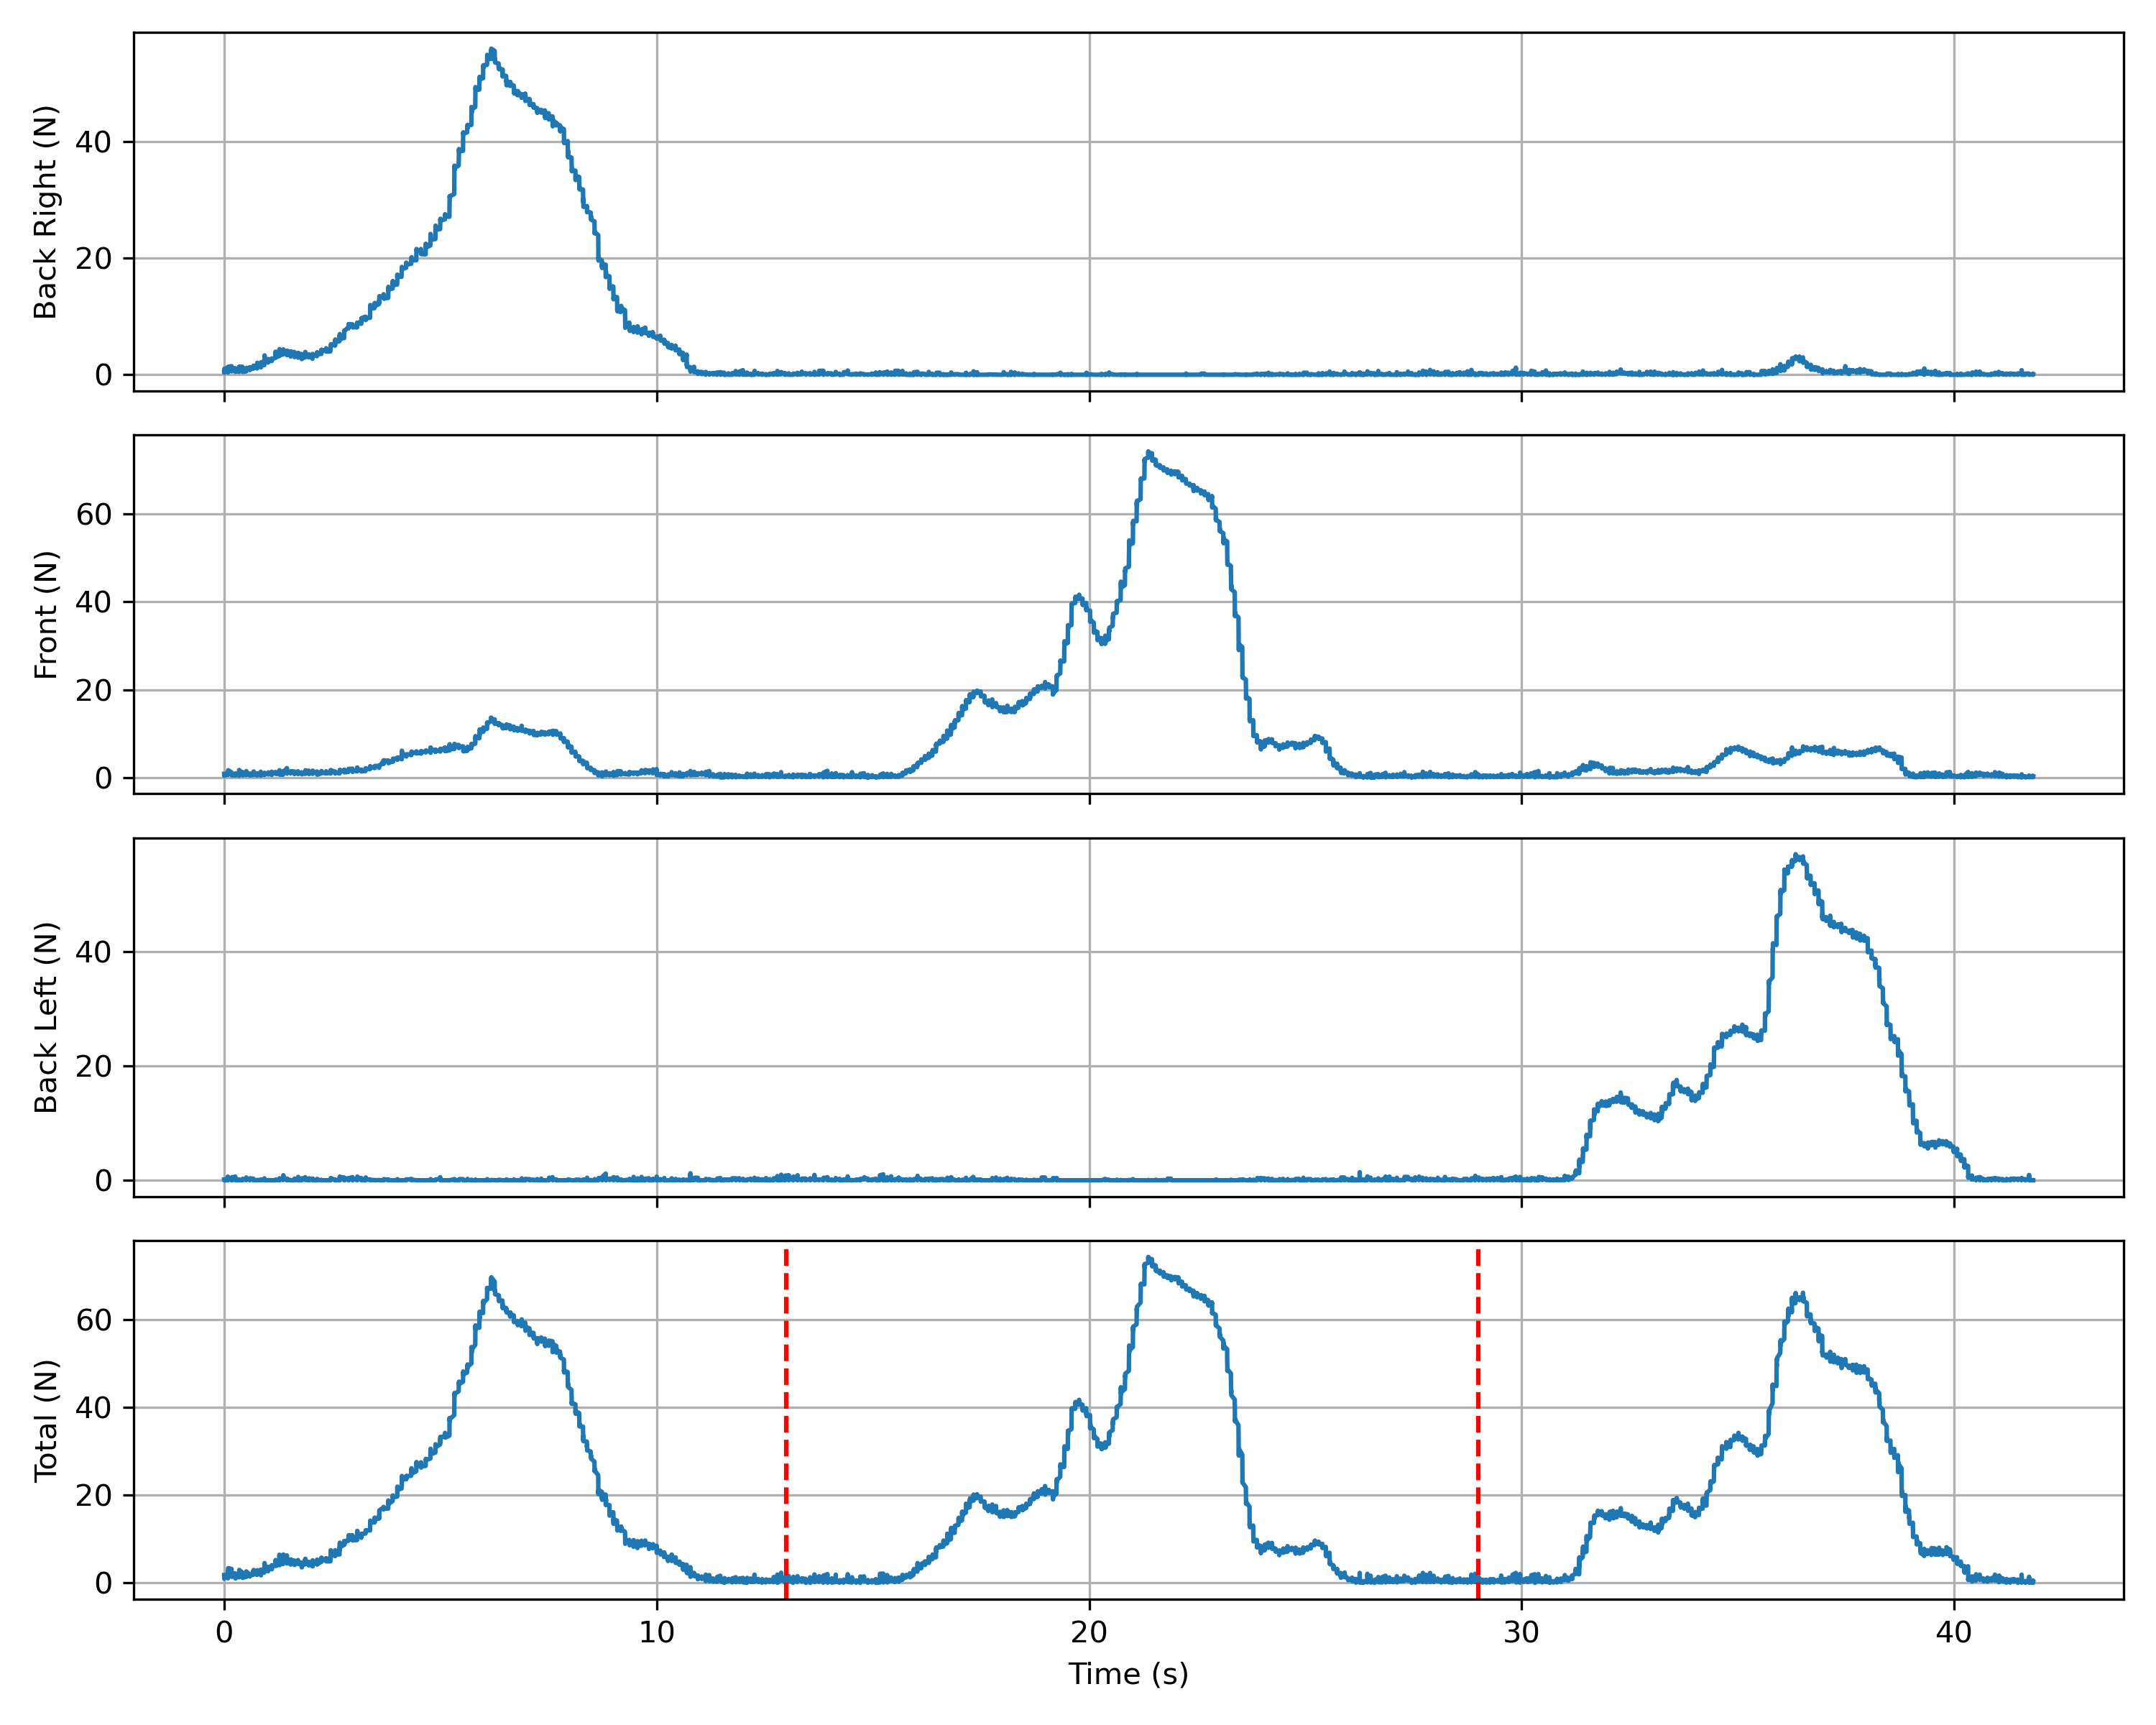
\includegraphics[width=0.8\textwidth]{figures/ForceDistributionGum.png}
    \caption{Vertical force output across three load cells during chewing with localized gum placement.  
    The red lines separate the three gum positions: back right, front, and back left.}
    \label{fig:force_distribution_gum}
\end{figure}

\subsection{Scalability and modularity}
A central goal of the project was to build a scalable platform for future modules such as a tongue, saliva pumps, and an esophagus. As described in 
Section~\ref{sec:mechanical_design}, the mechanical design already accommodates these additions, including space for internal cameras to observe the 
chewing process. A rendering of the proposed tongue module is shown in Figure~\ref{fig:tongue}. These design decisions were made in collaboration with 
project supervisor Benhui Dai.

\begin{figure}[H]
\centering
\begin{minipage}{.45\textwidth}
  \centering
  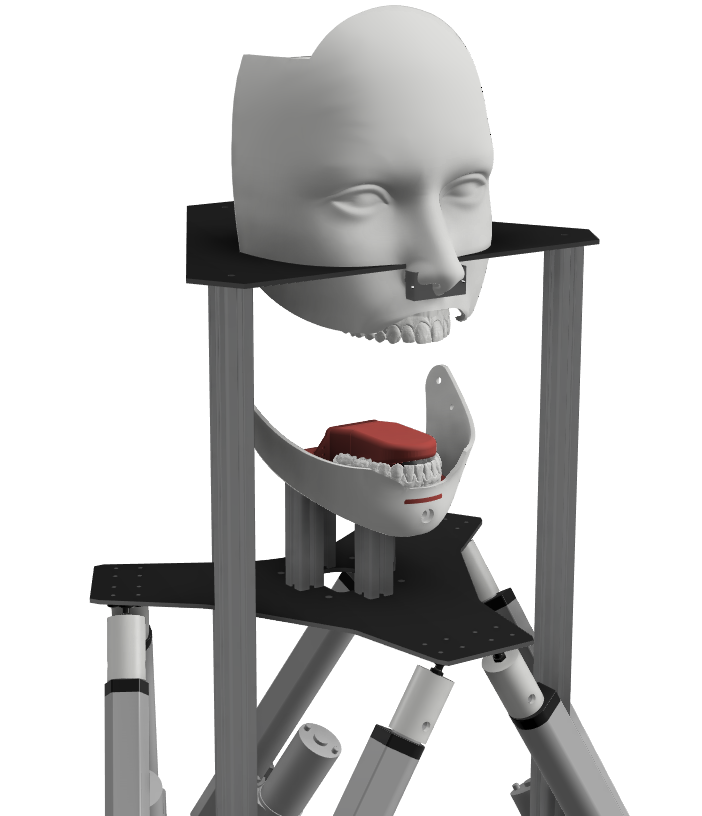
\includegraphics[height=5cm]{figures/tongue_front.png}
  \subcaption{}
  \label{fig:tongue_front}
\end{minipage}
\begin{minipage}{.45\textwidth}
  \centering
  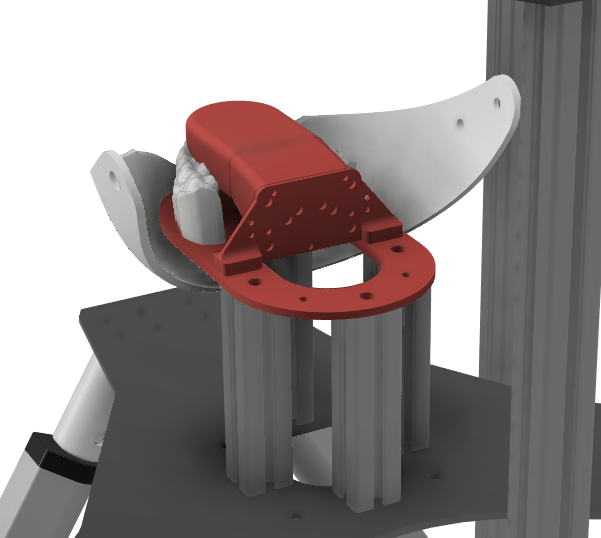
\includegraphics[height=5cm]{figures/tongue_back.png}
  \subcaption{}
  \label{fig:tongue_back}
\end{minipage}
\caption{Future tongue module rendering. (a) Front view, (b) Back view. }
\label{fig:tongue}
\end{figure}

The control system, detailed in Section~\ref{sec:control}, was developed with similar modularity in mind. Its finite-state machine architecture supports 
the easy integration of new components such as actuators and sensors for additional subsystems.

The robot's modularity also extends to the dental elements. Maxillary and mandibular teeth are mounted on replaceable acrylic adaptors, allowing for 
rapid testing of different dentitions. Combined with flexible trajectory loading, this makes the system suitable for a wide range of experimental and clinical scenarios.

\section{Discussion}
\subsection{Summary of findings}

\subsection{Limitations}
\begin{itemize}
    \item So far very big and heavy robot due to steel plates and big actuator \(\neq\) human jaw
    \item 3D printed teeth/jaw not strong enough to withstand the forces applied by the actuators
\end{itemize}

\subsection{Future work}
\begin{itemize}
    \item 3D printed jaw/teeth to be replaced by a more rigid material
    \item add a tongue module
    \item add a saliva module
    \item adapt state machine to coordinate the different modules
    \item add a camera to track the food
\end{itemize}

\section{Conclusion}

This project presented the design and development of a novel chewing robot capable of reproducing basic jaw motions using a Stewart platform. 
The mechanical architecture, control system, and data processing pipeline were developed with extensibility and modularity in mind, laying the 
groundwork for a more complete biomimetic mastication system.

The robot successfully replicates simplified human jaw trajectories using motion capture data and demonstrates the ability to apply significant 
occlusal forces. The modular control system and mechanical design allow for future integration of additional features, such as a tongue, saliva 
module, or esophagus. The inclusion of force sensing also enables basic safety mechanisms, and the current hardware supports a wide vertical 
range of motion suitable for chewing tasks.

Despite these achievements, the robot in its current form is not yet capable of full chewing functionality. Limitations in mechanical compliance, 
control accuracy, sensing precision, and tooth design prevent accurate and robust reproduction of natural mastication. Additionally, the current 
motion capture methodology introduces errors that limit the fidelity of recorded trajectories.

Nonetheless, the system serves as a strong foundation for future work. Improvements in control strategy, sensing, compliance, and anatomical 
fidelity—combined with more accurate motion datasets—will enable the robot to more closely replicate the biomechanics of human chewing. This 
work offers a promising starting point for research in food processing, oral biomechanics, and human-robot interaction involving mastication.


\newpage
\section{References}
\printbibliography[heading=none]

\section{Appendix}

\subsection{Real robot pictures}
\label{sec:real_pictures}
\begin{figure}[H]
    \centering
    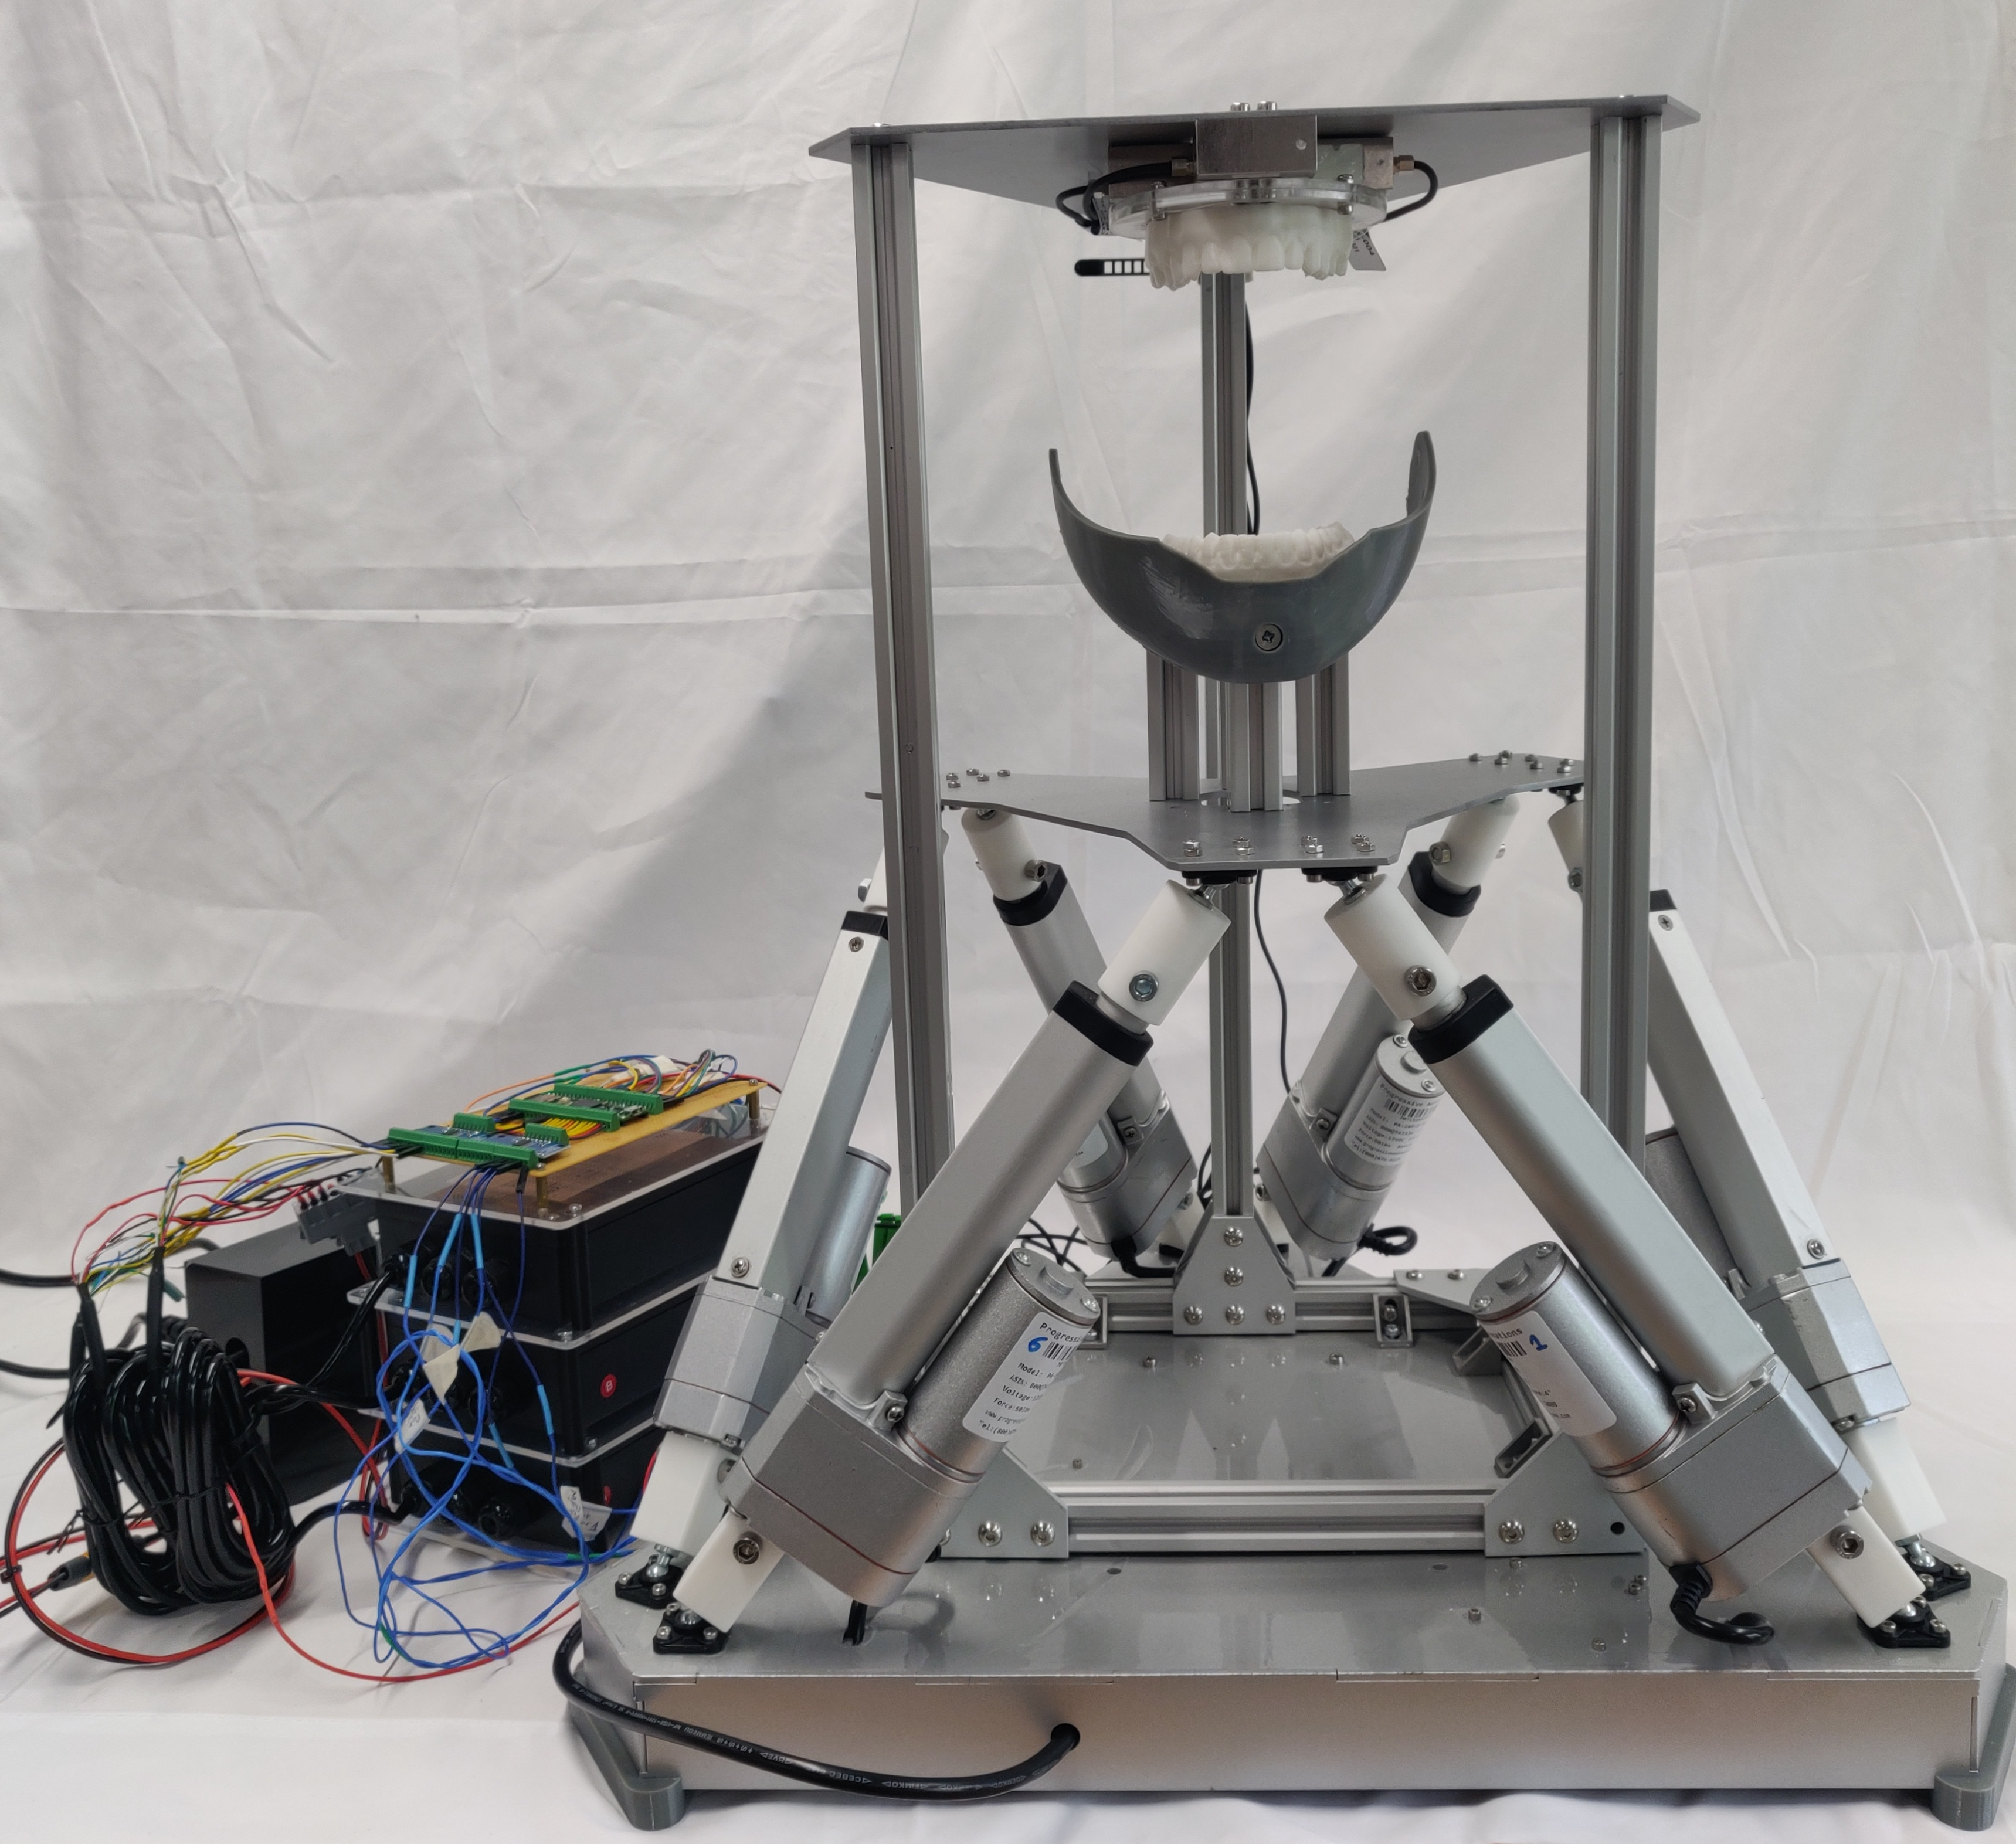
\includegraphics[width=0.8\textwidth]{figures/overview_real.jpg}
    \caption{Picture of the robot overview, including electronics on the left side.}
    \label{fig:overview_real}
\end{figure}

\begin{figure}[H]
    \centering
    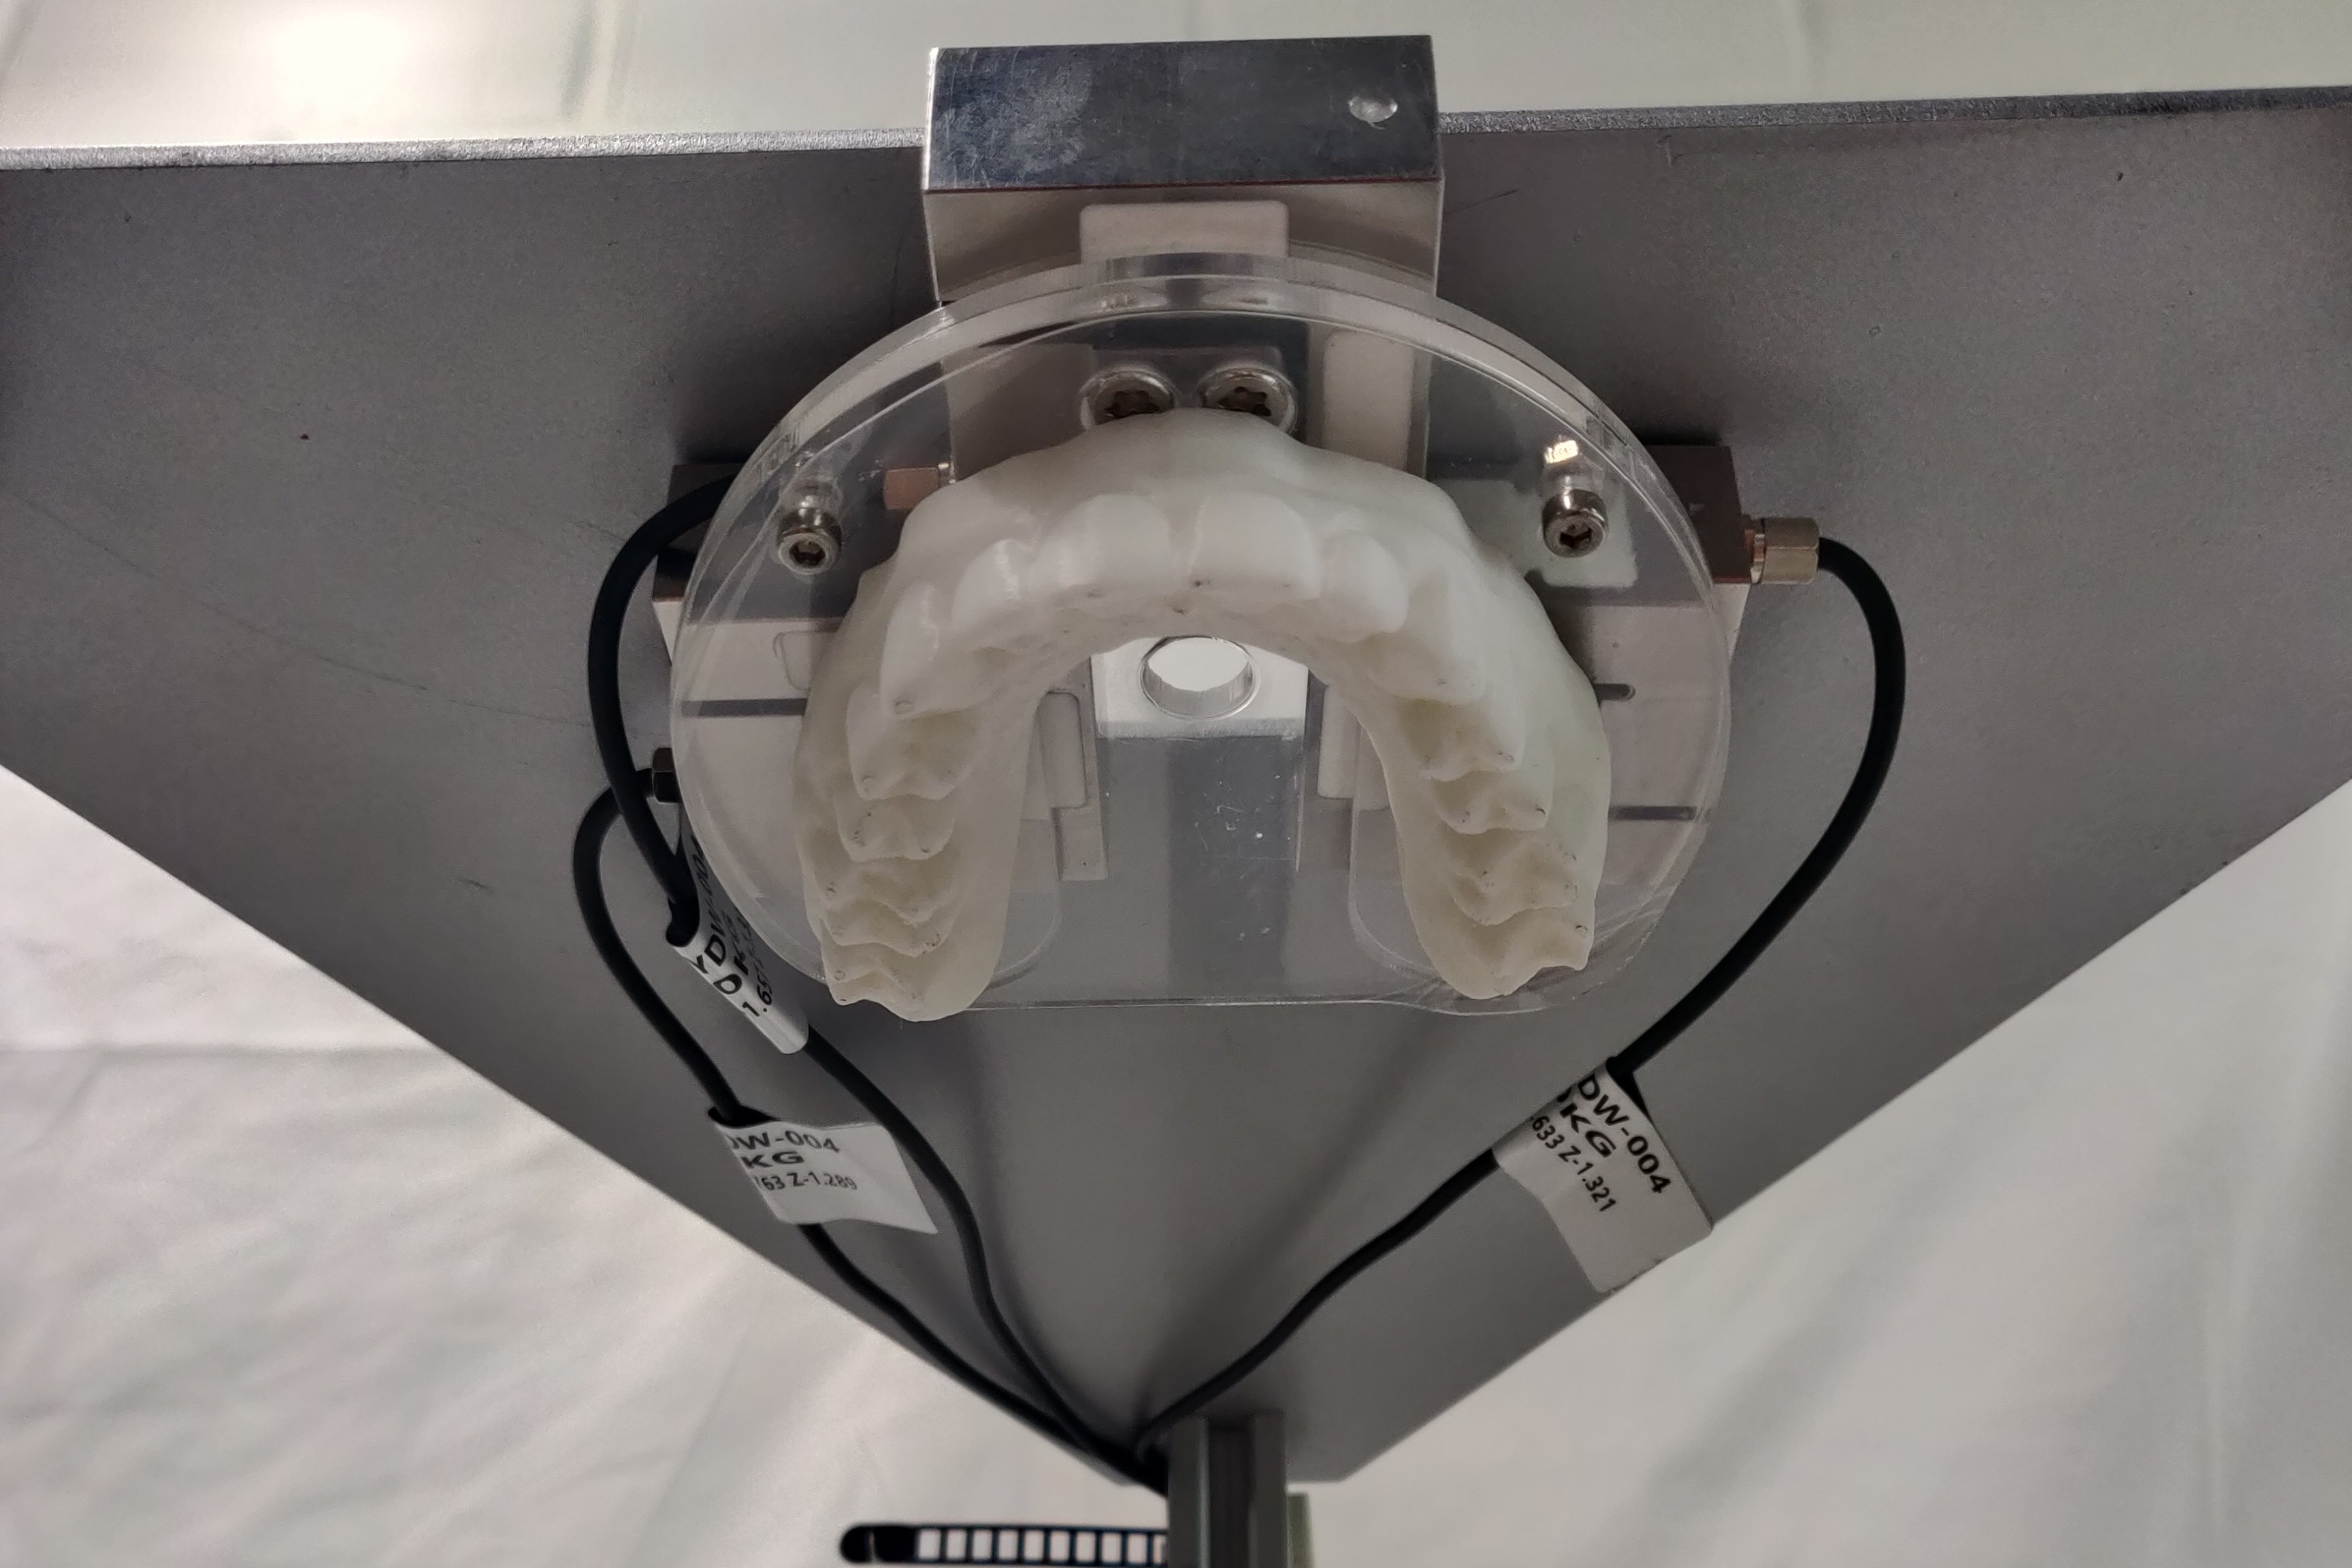
\includegraphics[width=0.6\textwidth]{figures/upper_jaw_close_up.jpg}
    \caption{Picture of the upper jaw close-up.}
    \label{fig:pic_upper_jaw_close_up}
\end{figure}

\begin{figure}[H]
    \centering
    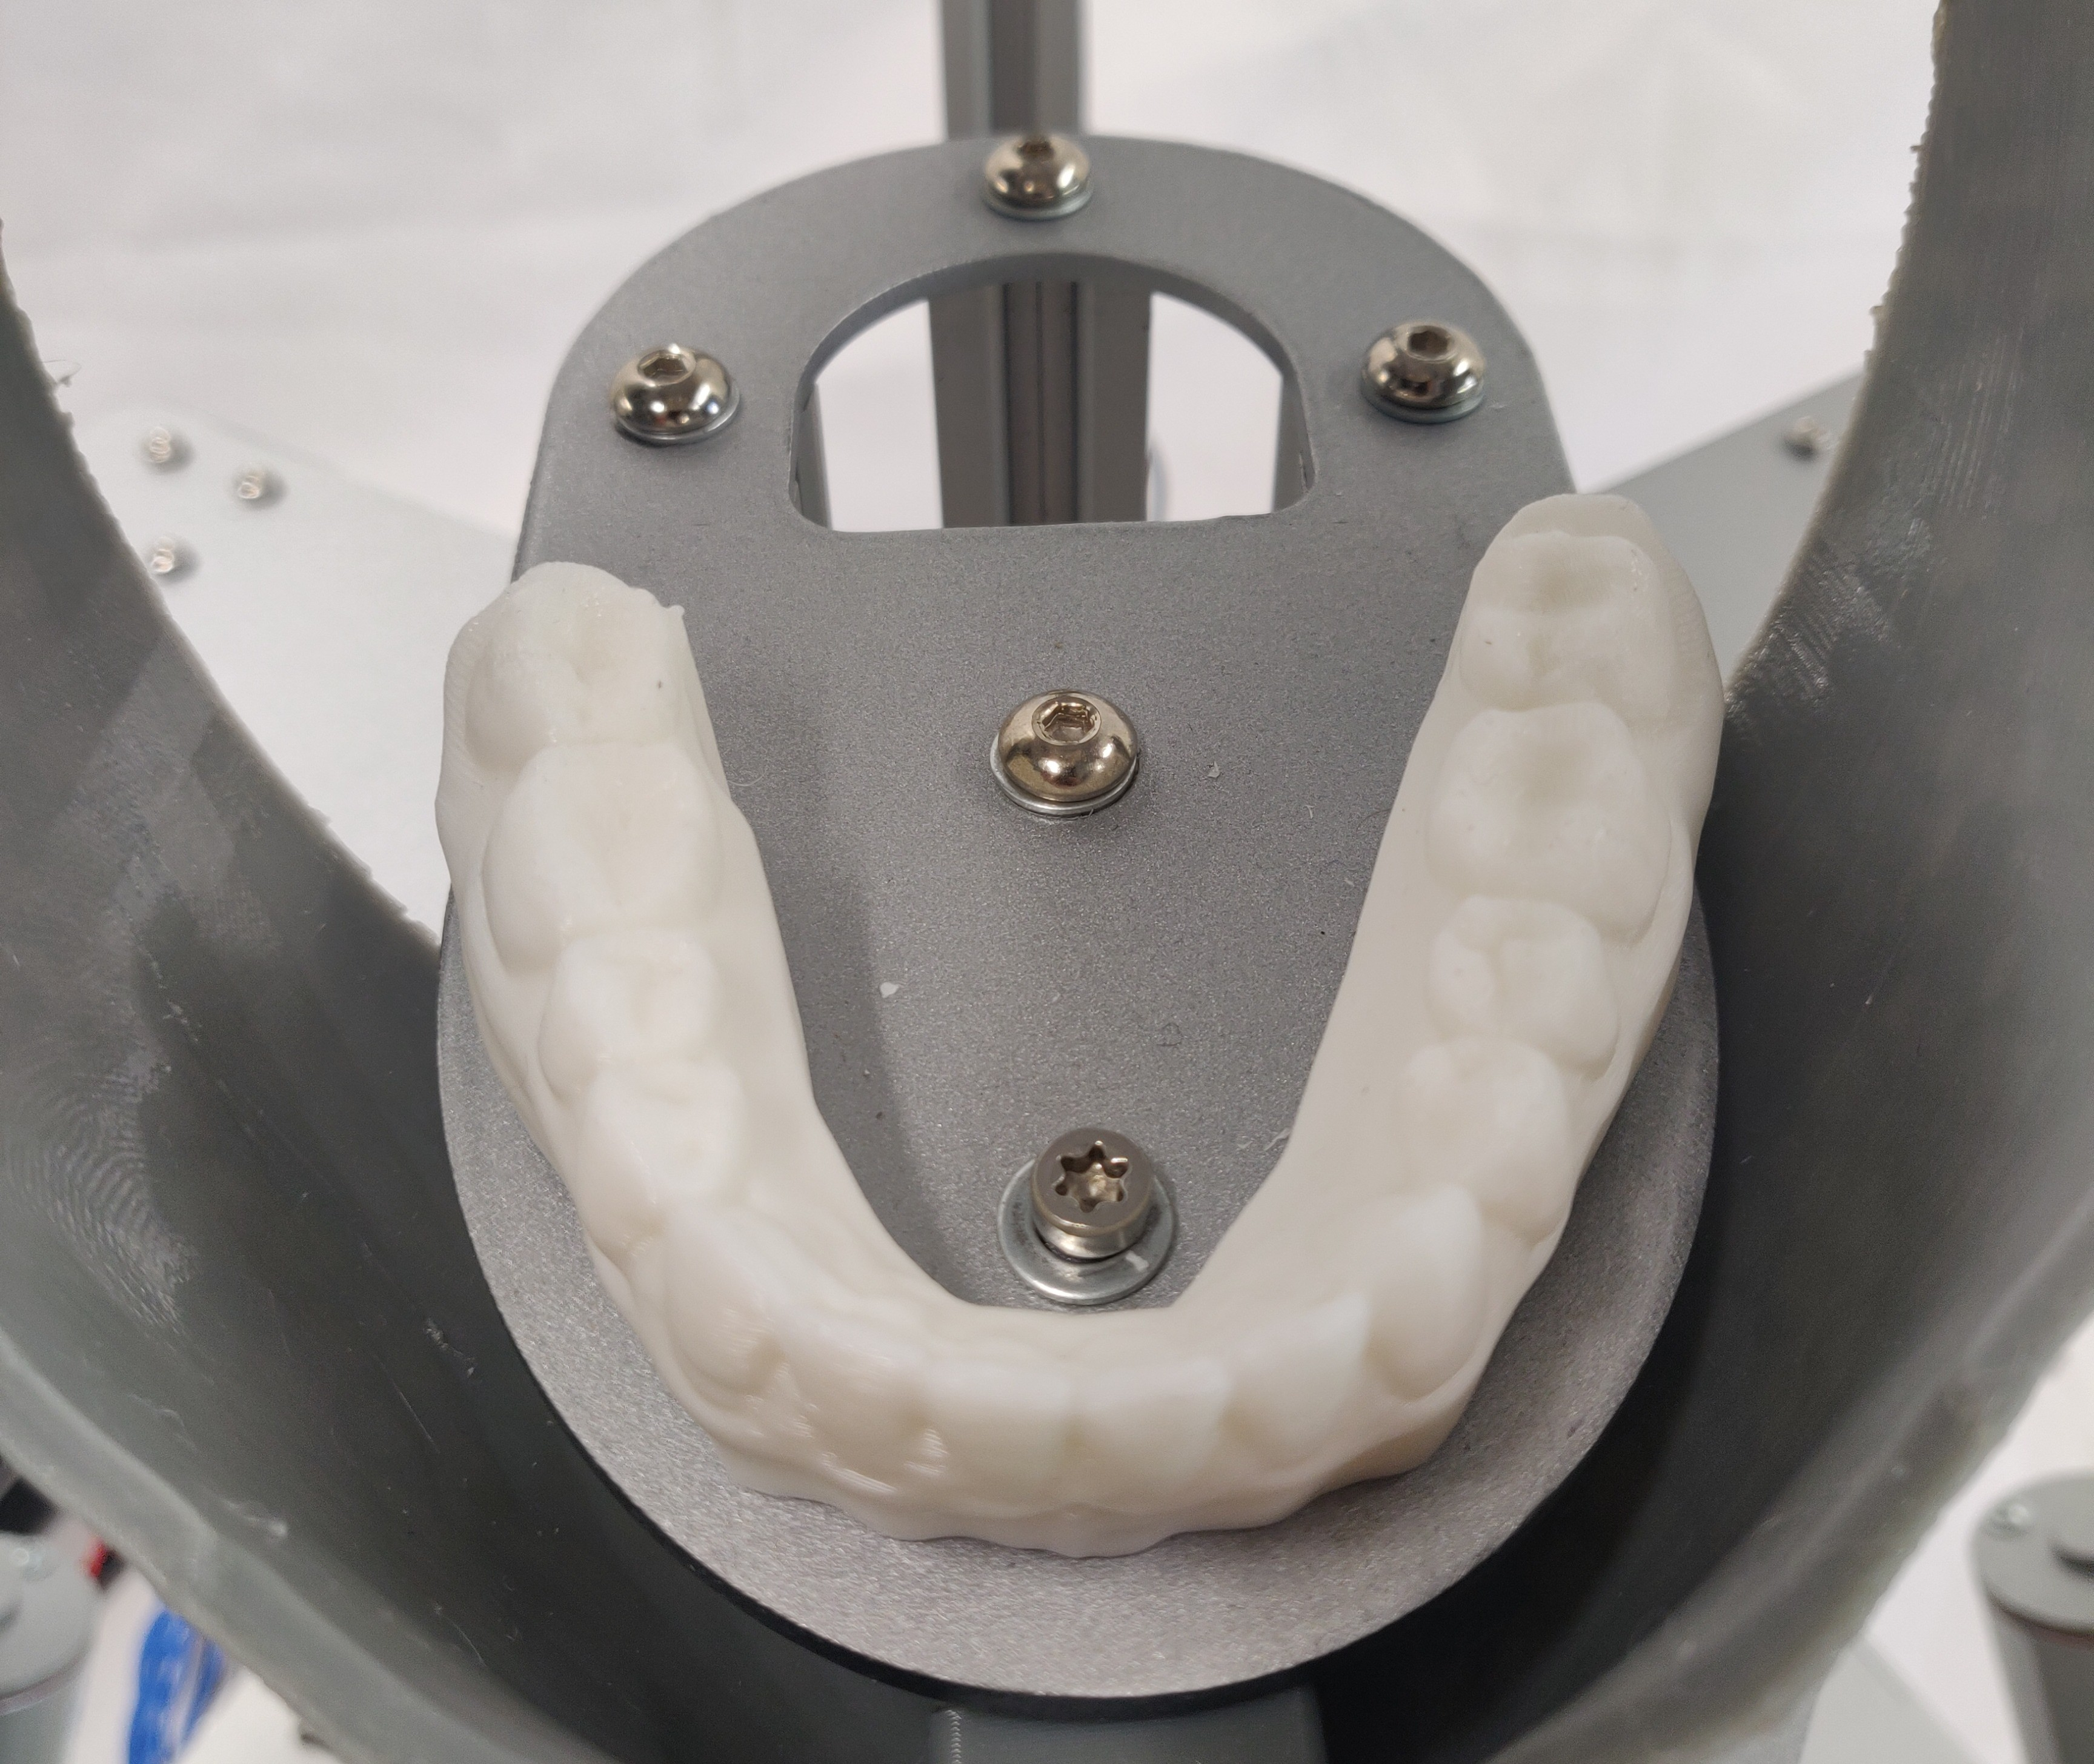
\includegraphics[width=0.6\textwidth]{figures/lower_jaw_close_up.jpg}
    \caption{Picture of the lower jaw close-up.}
    \label{fig:pic_lower_jaw_close_up}
\end{figure}

\begin{figure}[H]
    \centering
    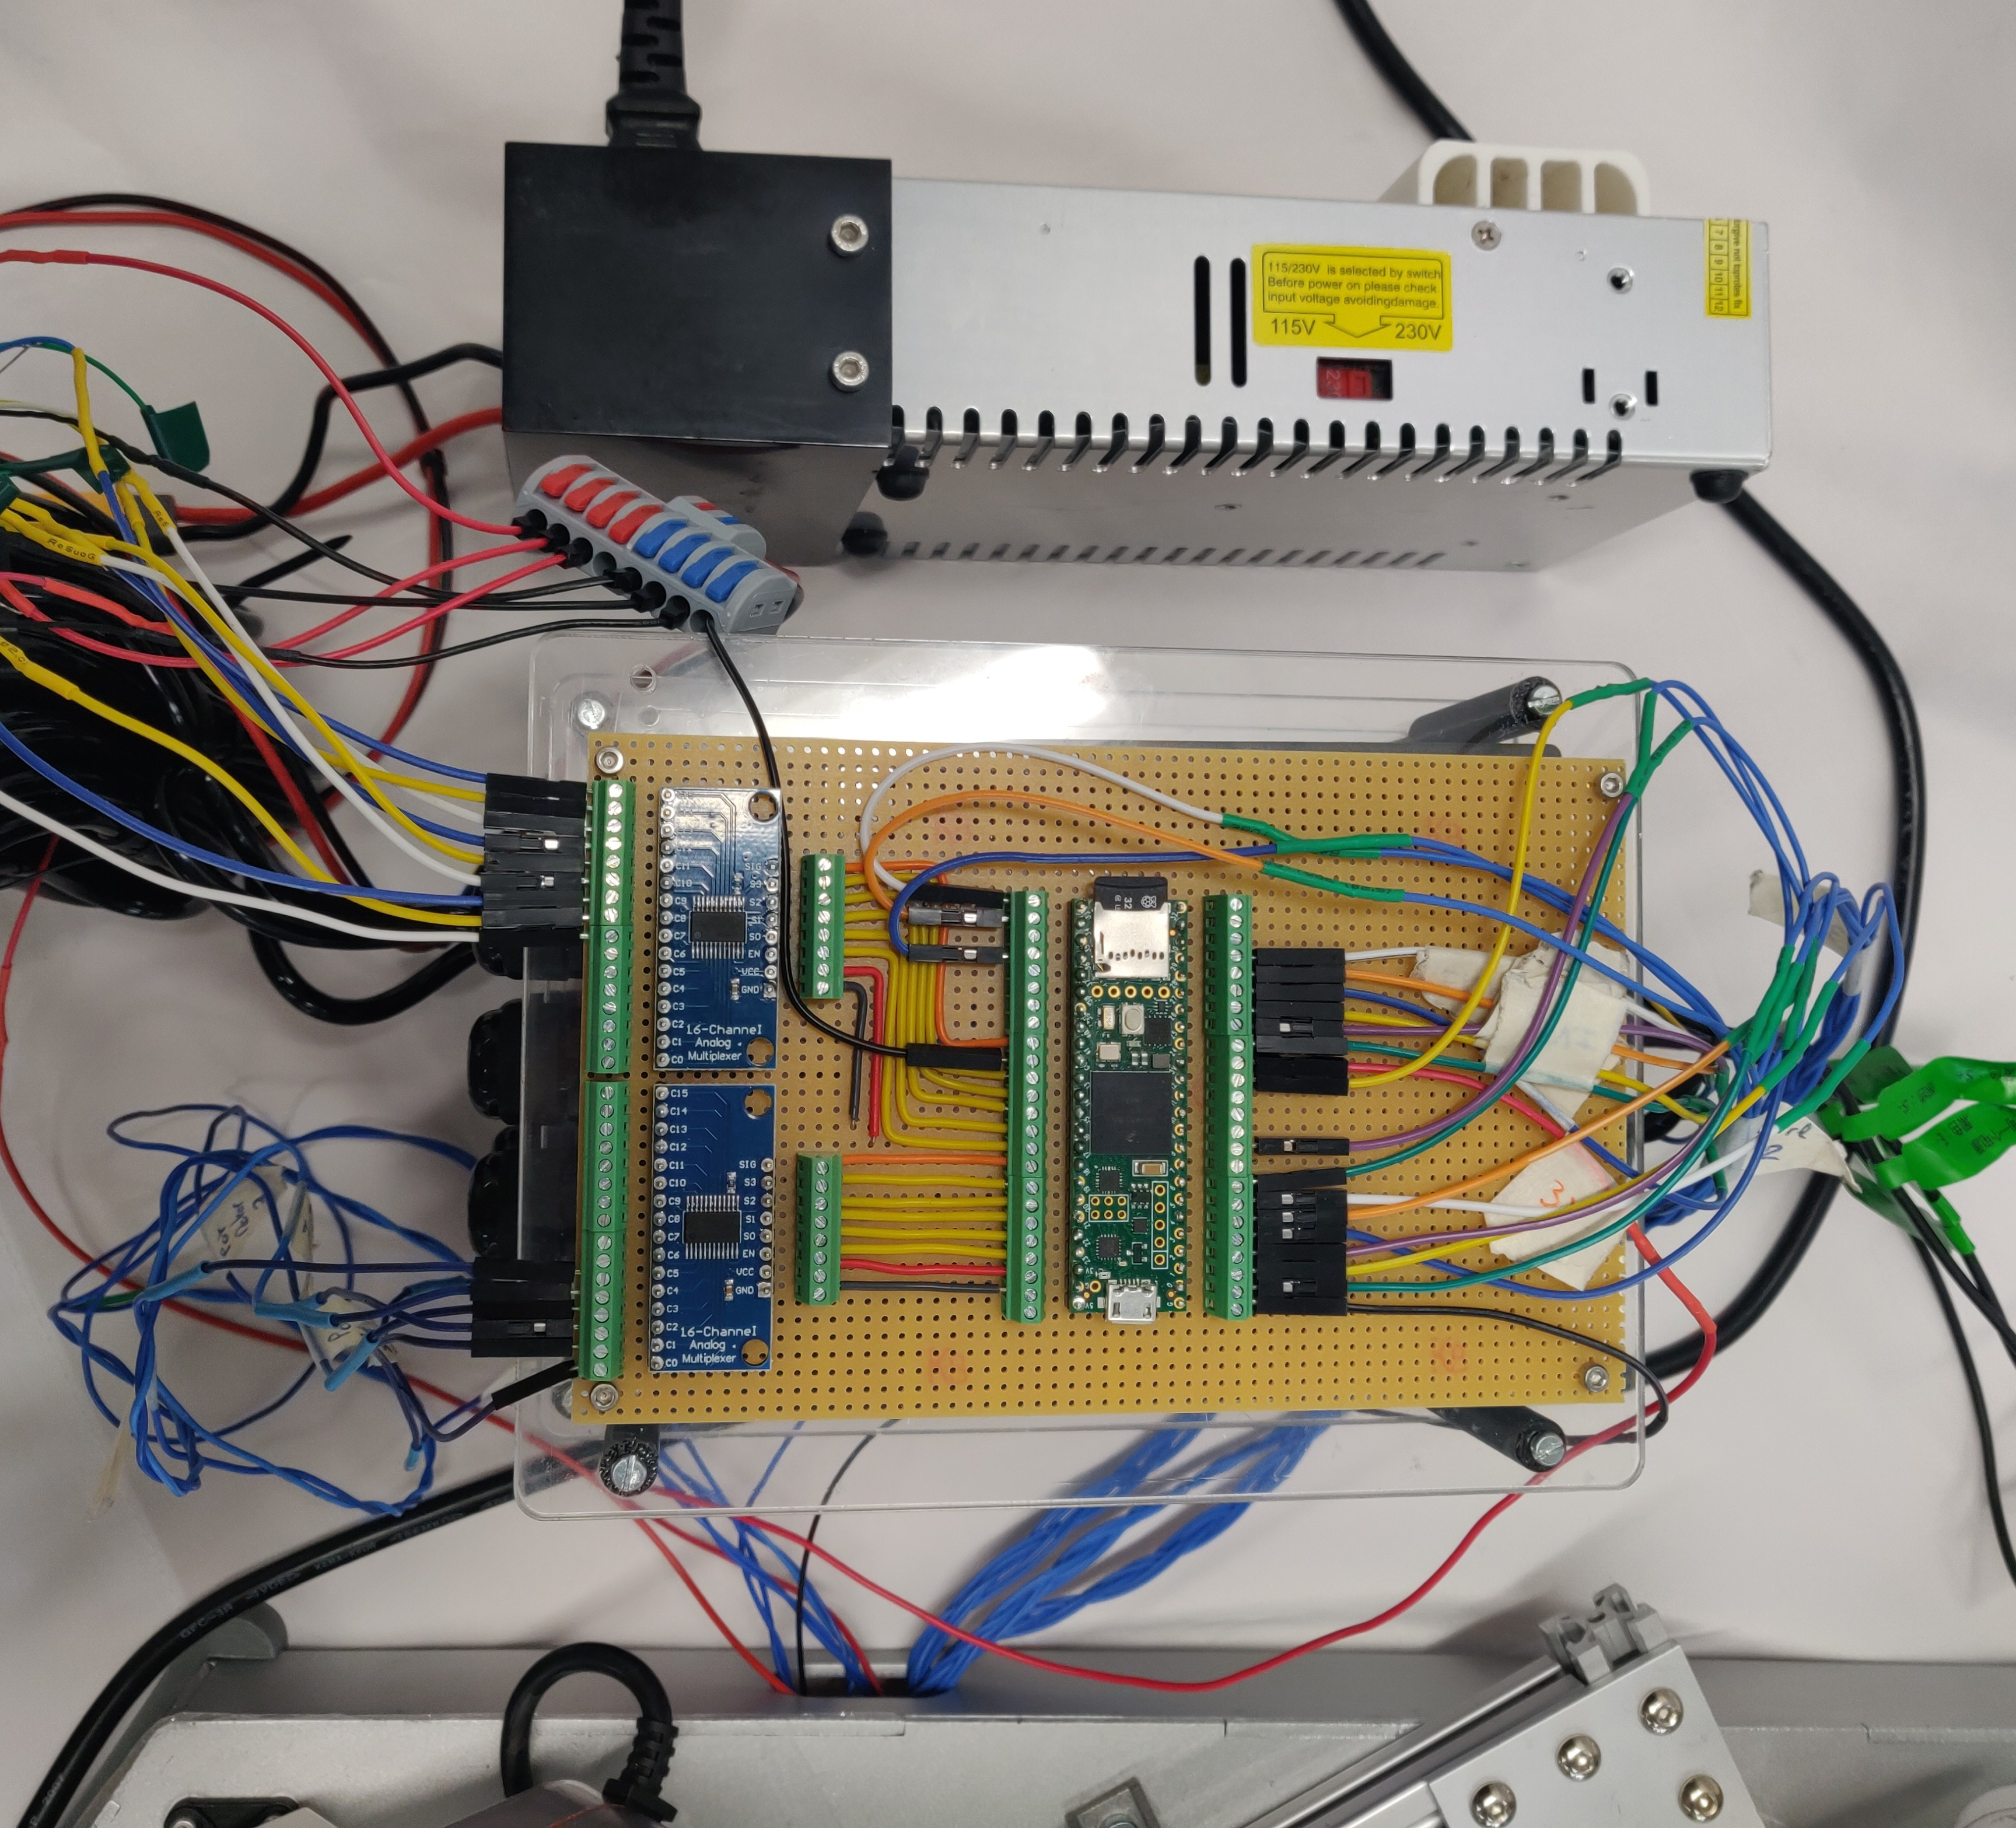
\includegraphics[width=0.7\textwidth]{figures/elec_close_up.jpg}
    \caption{Picture of the main electronics close-up.}
    \label{fig:pic_elec_close_up}
\end{figure}

\subsection{Electronics connections to Teensy~4.1}

\begin{figure}[H]
    \centering
    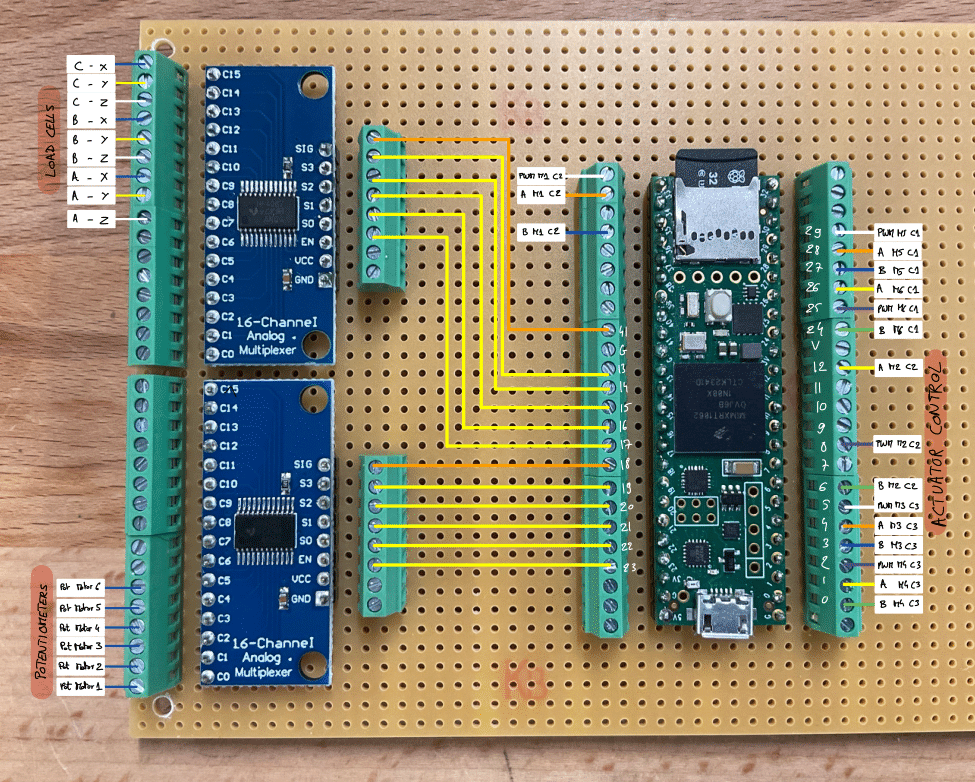
\includegraphics[width=\textwidth]{figures/elec_connections.png}
    \caption{Connections to Teensy~4.1. \textit{Notes: } "PWM M1 C2" refers to the PWM signal for motor 1 connected to controller number 2, 
    'A - X' refers to analog input for load cell A (front) axis X, "Pot Motor 1" refers to the potentiometer for motor 1.}
    \label{fig:connections_teensy}
\end{figure}

\begin{table}[h]
    \centering
    \begin{tabular}{|c|c|c|}
        \hline
        \textbf{Motor} & \textbf{Controller} & \textbf{Output} \\ \hline
        Motor 1 & \multirow{2}{*}{Controller 2} & Motor1 output \\ \cline{1-1} \cline{3-3}
        Motor 2 &  & Motor2 output \\ \hline
        Motor 3 & \multirow{2}{*}{Controller 3} & Motor1 output \\ \cline{1-1} \cline{3-3}
        Motor 4 &  & Motor2 output \\ \hline
        Motor 5 & \multirow{2}{*}{Controller 1} & Motor1 output \\ \cline{1-1} \cline{3-3}
        Motor 6 &  & Motor2 output \\ \hline
    \end{tabular}
    \caption{Motor-to-controller output connections.}
\end{table}

\end{document}